% !TeX program = pdflatex
% Báo cáo Seminar 1 – Môn Sinh trắc học
% Tệp tổng hợp độc lập theo đúng cấu trúc yêu cầu Seminar 1 (không chỉnh sửa các tệp cũ).
% Biên dịch: pdflatex report.tex -> biber report -> pdflatex report.tex -> pdflatex report.tex

\documentclass[oneside,a4paper,12pt]{extarticle}
% Lưu ý: đổi 12pt thành 14pt nếu muốn giữ đúng cỡ chữ của main.tex.

% Font tiếng Việt
\usepackage[T5]{fontenc}
\usepackage[utf8]{inputenc}
\DeclareTextSymbolDefault{\DH}{T1}

% Tài liệu tham khảo chuẩn IEEE (nhúng trực tiếp bằng thebibliography để pdflatex biên dịch không cần biber)
% \usepackage[style=ieee,backend=biber]{biblatex}
% \addbibresource{refs/references.bib}
\usepackage{xurl}
\usepackage[unicode]{hyperref}

% Chèn hình
\usepackage{graphicx}
\usepackage{float}
\usepackage{subcaption}
\graphicspath{ {images/} }

% Toán học và mã giả
\usepackage{amsmath}
\usepackage{algorithm}
\usepackage[noend]{algpseudocode}
\makeatletter
\def\BState{\State\hskip-\ALG@thistlm}
\makeatother

% Bảng biểu
\usepackage{multirow}
\usepackage{array}
\usepackage{booktabs}
\usepackage{longtable}
\newcolumntype{L}[1]{>{\raggedright\let\newline\\\arraybackslash\hspace{0pt}}m{#1}}
\newcolumntype{C}[1]{>{\centering\let\newline\\\arraybackslash\hspace{0pt}}m{#1}}
\newcolumntype{R}[1]{>{\raggedleft\let\newline\\\arraybackslash\hspace{0pt}}m{#1}}
\newcolumntype{P}[1]{>{\raggedright\arraybackslash}p{#1}}

% Định nghĩa ký hiệu cho bảng so sánh CFB (chỉ dùng ký hiệu, không màu)
\providecommand{\cOK}{\ensuremath{\surd}}       % đạt
\providecommand{\cNO}{\ensuremath{\times}}      % không đạt
\providecommand{\cPT}{\ensuremath{\sim}}        % đạt một phần
\providecommand{\cNA}{--}                       % bài báo không đánh giá
\providecommand{\cINF}{\ensuremath{^{\dagger}}} % suy luận của nhóm
\providecommand{\cCF}{\ensuremath{^{\ddagger}}} % các nguồn mâu thuẫn nhau
\ifdefined\cfbcolw\else\newlength{\cfbcolw}\fi

% Đổi tên mặc định tiếng Việt
\renewcommand{\figurename}{Hình}
\renewcommand{\tablename}{Bảng}
\renewcommand{\contentsname}{Mục lục}
\renewcommand{\listfigurename}{Danh sách hình}
\renewcommand{\listtablename}{Danh sách bảng}
\renewcommand{\appendixname}{Phụ lục}
\renewcommand{\refname}{Tài liệu tham khảo}

% Dãn dòng và thụt đầu dòng
\usepackage{setspace}
\onehalfspacing
\usepackage{indentfirst}

% Canh lề (giữ nguyên thông số của main.tex)
\usepackage[
  top=30mm,
  bottom=25mm,
  left=30mm,
  right=20mm,
  includefoot]{geometry}

% Trang bìa và hình vẽ TikZ
\usepackage{tikz}
\usetikzlibrary{calc,arrows.meta}
\newcommand\HRule{\rule{\textwidth}{1pt}}

\begin{document}

% =====================================================================
% 1. TRANG BÌA (Giữ nội dung gốc từ report/title/title.tex, bổ sung đủ yêu cầu Mục 3.1 Seminar 1)
% =====================================================================
\begin{titlepage}

\begin{center}

TRƯỜNG ĐẠI HỌC KHOA HỌC TỰ NHIÊN\\
\textbf{KHOA CÔNG NGHỆ THÔNG TIN}\\[0.5cm]
{\large \bfseries SEMINAR 1 --- MÔN SINH TRẮC HỌC}\\[0.8cm]

{\large \bfseries NHÓM 9}\\[0.2cm]
{\normalsize \bfseries Hoàng Ngọc -- 23120146}\\
{\normalsize \bfseries Võ Tất Toàn -- 23120097}\\
{\normalsize \bfseries Lê Đức Thành -- 23120165}\\
{\normalsize \bfseries Lê Quốc Hưng -- 23120270}\\
{\normalsize \bfseries Nguyễn Viết Toàn -- 23120096}\\[0.6cm]


\includegraphics[width=0.25\textwidth]{logo-khtn.png}\\[0.7cm]

{\normalsize \bfseries CHƯƠNG SÁCH PHÂN CÔNG}\\[0.15cm]
{\Large \bfseries Chương 19: Biometric System Security}\\[0.1cm]
{\small Andy Adler, \textit{Handbook of Biometrics}, Springer, 2008, tr.~381--402}\\[0.7cm]

{\normalsize \bfseries BÀI BÁO KHOA HỌC}\\[0.15cm]
{\large \bfseries FaceAnonyMixer: Cancelable Faces via Identity Consistent Latent Space Mixing}\\[0.15cm]
{\small M.~T.~Alam, F.~Shamshad, F.~Karray, and K.~Nandakumar}\\[0.45cm]

\begin{minipage}{0.92\textwidth}
\centering
\small
\begin{tabular}{@{}l@{\quad}l@{}}
\textbf{Đường dẫn bài báo:} & \url{https://arxiv.org/abs/2508.05636} \\
\textbf{Mã nguồn gốc:} & \url{https://github.com/talha-alam/faceanonymixer} \\
\textbf{Hội nghị -- Năm:} & IEEE Int. Joint Conf. Biometrics (IJCB), 2025 (tr.~1--10)
\end{tabular}
\end{minipage}

\begin{tikzpicture}[remember picture, overlay]
  \draw[line width = 2pt] ($(current page.north west) + (2cm,-2cm)$) rectangle ($(current page.south east) + (-1.5cm,2cm)$);
\end{tikzpicture}

\vfill
Tp. Hồ Chí Minh, tháng 11/2026

\end{center}
\pagenumbering{gobble}
\end{titlepage}

\clearpage
\pagenumbering{roman}

% =====================================================================
% PHẦN MỞ ĐẦU: MỤC LỤC, DANH MỤC (Nguồn nguyên văn: report/Appendix/glossary.tex)
% =====================================================================
\phantomsection
\addcontentsline{toc}{section}{Mục lục}
\tableofcontents

\clearpage
\phantomsection
\section*{Danh mục các từ viết tắt}
\addcontentsline{toc}{section}{Danh mục các từ viết tắt}

{\small
\renewcommand{\theHtable}{glossary.abbr.\arabic{table}}
\begin{longtable}{r l >{\raggedright\arraybackslash}p{10.6cm}}
\toprule
\textbf{STT} & \textbf{Viết tắt} & \textbf{Tên đầy đủ} \\
\midrule
\endfirsthead
\toprule
\textbf{STT} & \textbf{Viết tắt} & \textbf{Tên đầy đủ} \\
\midrule
\endhead
\bottomrule
\endfoot
1 & AI & Artificial Intelligence -- Trí tuệ nhân tạo \\
2 & API & Application Programming Interface -- Giao diện lập trình ứng dụng \\
3 & AUC & Area Under the Curve -- Diện tích dưới đường cong ROC \\
4 & CanFG & Cancelable Face Generator -- Bộ sinh khuôn mặt có thể hủy \\
5 & CFB & Cancelable Face Biometrics -- Sinh trắc học khuôn mặt có thể hủy \\
6 & DL & Deep Learning -- Học sâu \\
7 & e4e & Encoder for Editing -- Bộ mã hóa phục vụ chỉnh sửa \\
8 & EER & Equal Error Rate -- Tỷ lệ lỗi cân bằng \\
9 & FaRL & Facial Representation Learning -- Học biểu diễn khuôn mặt đa phương thức \\
10 & FFHQ & Flickr-Faces-HQ -- Tập dữ liệu ảnh khuôn mặt độ phân giải cao \\
11 & FID & Fréchet Inception Distance -- Khoảng cách Fréchet Inception \\
12 & FMR & False Match Rate -- Tỷ lệ chấp nhận nhầm \\
13 & FNMR & False Non-Match Rate -- Tỷ lệ từ chối nhầm \\
14 & FR & Face Recognition -- Nhận dạng khuôn mặt \\
15 & GAN & Generative Adversarial Network -- Mạng đối sinh \\
16 & ISO/IEC & International Organization for Standardization / International Electrotechnical Commission -- Tổ chức Tiêu chuẩn hóa Quốc tế / Ủy ban Kỹ thuật Điện Quốc tế \\
17 & MLP & Multi-Layer Perceptron -- Mạng nơ-ron đa tầng \\
18 & MTCNN & Multi-task Cascaded Convolutional Networks -- Mạng tích chập phân tầng đa nhiệm \\
19 & PSR & Protection Success Rate -- Tỷ lệ bảo vệ thành công \\
20 & SOTA & State-of-the-Art -- Tiên tiến nhất hiện nay \\
21 & StyleGAN & Style-based Generative Adversarial Network -- Mạng đối sinh dựa trên phong cách \\
22 & U-Net & U-shaped Convolutional Network -- Mạng tích chập kiến trúc chữ U \\
23 & VID & Virtual Identity -- Danh tính ảo \\
\end{longtable}
\addtocounter{table}{-1}
}

\clearpage
\phantomsection
\section*{Danh mục các thuật ngữ}
\addcontentsline{toc}{section}{Danh mục các thuật ngữ}

{\small
\renewcommand{\theHtable}{glossary.terms.\arabic{table}}
\begin{longtable}{r >{\raggedright\arraybackslash}p{5.2cm} >{\raggedright\arraybackslash}p{8.0cm}}
\toprule
\textbf{STT} & \textbf{Tiếng Anh} & \textbf{Tiếng Việt} \\
\midrule
\endfirsthead
\toprule
\textbf{STT} & \textbf{Tiếng Anh} & \textbf{Tiếng Việt} \\
\midrule
\endhead
\bottomrule
\endfoot
1 & Anonymity & Tính ẩn danh \\
2 & Artifact & Biến dạng giả / Nhiễu nhân tạo \\
3 & Attack Tree & Cây tấn công \\
4 & Attribute Preservation & Bảo toàn thuộc tính (phi danh tính) \\
5 & Augmentation & Tăng cường dữ liệu / Tạo biến thể \\
6 & Biometric System Security & Bảo mật hệ thống sinh trắc học \\
7 & Black-box & Kịch bản hộp đen \\
8 & Cancelable Biometrics & Sinh trắc học có thể hủy \\
9 & Confidence Score & Điểm tin cậy (tương đồng) \\
10 & Control Grid & Lưới điểm neo / Lưới điều khiển \\
11 & Cross-matching & Đối chiếu chéo (liên kết danh tính) \\
12 & Disentanglement & Tách biệt thuộc tính (trong không gian tiềm ẩn) \\
13 & Distortion Scheme & Lược đồ biến dạng \\
14 & Enrollment & Pha đăng ký mẫu sinh trắc \\
15 & Face Morphing & Lai ghép khuôn mặt \\
16 & Feature-space & Không gian đặc trưng \\
17 & GAN Inversion & Đảo ngược GAN (chiếu ảnh vào không gian tiềm ẩn) \\
18 & Grid Morphing & Biến dạng lưới hình học \\
19 & Hill-Climbing & Thuật toán leo đồi \\
20 & Identity Preservation & Bảo toàn danh tính \\
21 & Image Morphing & Biến dạng ảnh / Lai ghép ảnh \\
22 & Image-space & Không gian ảnh (thô) \\
23 & Irreversibility & Tính không thể đảo ngược \\
24 & Key Mapping & Ánh xạ khóa \\
25 & Latent Code & Mã tiềm ẩn \\
26 & Latent Space & Không gian tiềm ẩn \\
27 & Loss Function & Hàm mất mát \\
28 & Na\"ive Mixing & Phép trộn thô / Trộn khởi tạo \\
29 & Optimization Loop & Vòng lặp tối ưu hóa \\
30 & Performance Preservation & Bảo toàn hiệu năng (nhận dạng) \\
31 & Pre-trained & Tiền huấn luyện \\
32 & Protected Face & Khuôn mặt được bảo vệ \\
33 & Random Seed & Hạt giống ngẫu nhiên \\
34 & Revocability & Tính khả hủy (thu hồi và cấp lại) \\
35 & Revocable Biometrics & Sinh trắc học có thể thu hồi / hủy \\
36 & Skip-connection & Liên kết tắt \\
37 & Style Mixing & Hòa trộn phong cách \\
38 & Test-time Optimization & Tối ưu hóa ở pha suy luận \\
39 & Thin-Plate Spline & Nội suy bản mỏng \\
40 & Undistort & Giải biến dạng ngược \\
41 & Unlinkability & Tính không thể liên kết \\
42 & Warping & Biến dạng hình học ảnh \\
\end{longtable}
\addtocounter{table}{-1}
}

\clearpage
\phantomsection
\section*{Danh mục các ký hiệu}
\addcontentsline{toc}{section}{Danh mục các ký hiệu}

{\small
\renewcommand{\theHtable}{glossary.sym.\arabic{table}}
\begin{longtable}{r l >{\raggedright\arraybackslash}p{8.8cm}}
\toprule
\textbf{STT} & \textbf{Ký hiệu} & \textbf{Ý nghĩa và vai trò} \\
\midrule
\endfirsthead
\toprule
\textbf{STT} & \textbf{Ký hiệu} & \textbf{Ý nghĩa và vai trò} \\
\midrule
\endhead
\bottomrule
\endfoot
1 & $\mathcal{X}$ & Không gian ảnh khuôn mặt. \\
2 & $\mathcal{K}$ & Không gian khóa có thể hủy. \\
3 & $\mathcal{W}^+$ & Không gian tiềm ẩn trung gian phân tầng của StyleGAN2. \\
4 & $\mathbf{x}_r,\; \mathbf{x}_p \in \mathcal{X}$ & Ảnh khuôn mặt thật đầu vào và ảnh được bảo vệ đầu ra. \\
5 & $\mathbf{k} \in \mathcal{K}$ & Khóa bí mật dùng làm hạt giống ngẫu nhiên. \\
6 & $\mathbf{z}_r,\; \mathbf{z}_f,\; \mathbf{z}_p \in \mathcal{W}^+$ & Mã tiềm ẩn của ảnh thật, mã sinh từ khóa và mã sau khi hòa trộn. \\
7 & $\mathbf{F} : \mathcal{X} \times \mathcal{X} \rightarrow \{0, 1\}$ & Bộ so khớp khuôn mặt ($1$: cùng người $\mathbf{x}_1 \equiv \mathbf{x}_2$; $0$: khác người $\mathbf{x}_1 \not\equiv \mathbf{x}_2$). \\
8 & $\mathbf{G} : \mathcal{X} \times \mathcal{K} \rightarrow \mathcal{X}$ & Bộ sinh khuôn mặt có thể hủy cần xây dựng ($\mathbf{x}_p = \mathbf{G}(\mathbf{x}_r, \mathbf{k})$). \\
9 & $\mathbf{S} : \mathcal{K} \rightarrow \mathcal{W}^+$ & Hàm ánh xạ khóa $\mathbf{k}$ sang mã tiềm ẩn giả lập $\mathbf{z}_f$. \\
10 & $\mathbf{E} : \mathcal{X} \rightarrow \mathcal{W}^+$ & Bộ mã hóa đảo ngược \textit{e4e} chiếu ảnh thật $\mathbf{x}_r$ sang mã tiềm ẩn $\mathbf{z}_r$. \\
11 & $\mathbf{M} : \mathcal{W}^+ \times \mathcal{W}^+ \rightarrow \mathcal{W}^+$ & Hàm hòa trộn $\mathbf{z}_r$ và $\mathbf{z}_f$ thành mã tiềm ẩn trộn $\mathbf{z}_p$. \\
12 & $\mathbf{D} : \mathcal{W}^+ \rightarrow \mathcal{X}$ & Bộ sinh StyleGAN2 tiền huấn luyện giải mã mã tiềm ẩn về ảnh khuôn mặt. \\
13 & $\mathbf{I},\; \mathbf{A}$ & Bộ trích xuất đặc trưng danh tính (ArcFace) và phi danh tính (FaRL). \\
14 & $\mathcal{L}_{\text{anon}}, \mathcal{L}_{\text{idp}}, \mathcal{L}_{\text{attr}}$ & Các hàm mất mát ẩn danh, bảo toàn danh tính và bảo toàn thuộc tính. \\
15 & $I(x, y),\; I'$ & Ảnh khuôn mặt gốc và ảnh mẫu sống khi xác thực. \\
16 & $\mathbf{p}_{i,j},\; \Delta \mathbf{p}_{i,j}(\mathbf{k})$ & Tọa độ điểm nút lưới điều khiển và độ dịch chuyển theo khóa $\mathbf{k}$. \\
17 & $\mathcal{T}_{\mathbf{k}},\; \mathcal{T}_{\mathbf{k}}^{-1}$ & Phép biến đổi tọa độ liên tục theo khóa $\mathbf{k}$ và ánh xạ ngược. \\
18 & $I_{\mathbf{k}},\; I_{\text{key}},\; I_p$ & Ảnh sau biến dạng lưới, ảnh tham chiếu theo khóa và ảnh sau pha trộn lai ghép. \\
19 & $\alpha \in (0, 1)$ & Hệ số pha trộn tuyến tính trong lai ghép khuôn mặt. \\
20 & $\mathcal{E}(\cdot),\; s(\cdot, \cdot),\; \tau$ & Bộ trích xuất đặc trưng chuẩn, hàm đo độ tương đồng và ngưỡng quyết định xác thực. \\
\end{longtable}
\addtocounter{table}{-1}
}

\clearpage
\phantomsection
\addcontentsline{toc}{section}{\listtablename}
\listoftables

\vspace{1em}
\phantomsection
\addcontentsline{toc}{section}{\listfigurename}
\listoffigures

\clearpage
\pagenumbering{arabic}

% =====================================================================
% TC1. KỸ THUẬT TRONG CHƯƠNG SÁCH
% Nguồn nguyên văn: report/chapter1/1.1-summary.tex (dòng 1--44)
% =====================================================================
\section{Kỹ thuật trong chương sách}
\label{sec:tc1}

\subsection{Tổng quan chương sách}
\label{sec:tong-quan}
Chương 19: \textit{Bảo mật hệ thống sinh trắc học} trình bày bởi tác giả Andy Adler trong giáo trình \textit{Handbook of Biometrics} \cite{adler2008} phân tích hệ thống các rủi ro an ninh và quyền riêng tư. Nội dung chương triển khai theo bốn nội dung chính từ Mục~19.1 đến Mục~19.6:
\begin{itemize}\setlength{\itemsep}{2pt}\setlength{\parskip}{0pt}
    \item \textbf{Tổng quan lỗ hổng và quyền riêng tư (Mục~19.1--19.2):} Phân loại các tấn công vào hệ thống sinh trắc học và chỉ rõ ba thách thức riêng tư cốt lõi (không bí mật, không thể thu hồi và nguy cơ sử dụng thứ cấp).
    \item \textbf{Lỗ hổng theo mô-đun và cây tấn công (Mục~19.3):} Phân tích điểm yếu tại từng khâu trong dây chuyền nhận dạng và mô hình hóa chuỗi khai thác bằng cây tấn công.
    \item \textbf{Tấn công tái tạo ảnh (Mục~19.4):} Chỉ ra nguy cơ khôi phục ảnh sinh trắc gốc từ mẫu lưu trữ hoặc từ điểm số so khớp trả về.
    \item \textbf{Các lược đồ bảo vệ mẫu (Mục~19.5 và 19.6):} Trình bày các hướng bảo vệ mẫu gồm sinh trắc học có thể hủy, mã hóa sinh trắc học và đo lường hàm lượng thông tin sinh trắc.
\end{itemize}

Trong bảo mật sinh trắc học, nhận dạng mặt thường được sử dụng rất nhiều trong các bước xác thực của rất nhiều ứng dụng lớn bởi sự tiện lợi và khả năng chính xác. Khác với sử dụng mật khẩu, khuôn mặt thường gắn liền với một người và không thể thay thế được, vì vậy sinh trắc học có thể hủy được phát triển như là một giải pháp cho nhu cầu bảo mật.

Các phương pháp sử dụng đặc trưng khuôn mặt có thể hủy được phát triển nhiều nhất. Mục tiêu chung của bài toán bảo mật xác định ``\textbf{Làm sao có thể tạo ra các mẫu/ảnh được bảo vệ mà vẫn giữ được khả năng nhận dạng trên hệ thống ?}''. Các phương pháp sử dụng đặc trưng mặt hiện nay sẽ cố gắng biến đổi khuôn mặt theo một mẫu hoặc phép biến đổi không thể tái tạo, vẫn giữ khả năng xác thực trong khi không bị lộ ảnh gốc. Có thể chia các phương pháp theo hai hướng dựa trên không gian thao tác, bao gồm (1) Không gian đặc trưng và (2) Không gian ảnh thô.

Để làm cơ sở đánh giá và so sánh các kỹ thuật ở các phần sau, Bảng~\ref{tab:core-concepts} tóm tắt bốn tiêu chuẩn bảo vệ mẫu sinh trắc học theo chuẩn ISO/IEC 24745 \cite{iso24745} cùng các độ đo hiệu năng và bảo mật nền tảng.

\begin{table}[H]
\centering
\caption[Các khái niệm và độ đo nền tảng về sinh trắc học có thể hủy]{Các khái niệm và độ đo nền tảng dùng để đánh giá, so sánh phương pháp sinh trắc học có thể hủy.}
\label{tab:core-concepts}
\begin{spacing}{1.08}
\footnotesize
\setlength{\tabcolsep}{4pt}
\begin{tabular}{@{}P{4.4cm}P{10.6cm}@{}}
\toprule
\textbf{Khái niệm / Độ đo} & \textbf{Ý nghĩa và vai trò trong đánh giá} \\
\midrule
\textbf{Tính khả hủy} (ISO/IEC 24745) & Cho phép thu hồi mẫu bị lộ và cấp lại mẫu mới bằng cách thay đổi khóa mà không cần thay đổi khuôn mặt gốc. \\
\addlinespace[3pt]
\textbf{Tính không thể liên kết} (ISO/IEC 24745) & Các mẫu bảo vệ tạo từ cùng một người với những khóa khác nhau không thể đối chiếu chéo giữa các ứng dụng. \\
\addlinespace[3pt]
\textbf{Tính không thể đảo ngược} (ISO/IEC 24745) & Không thể khôi phục ảnh hoặc danh tính gốc từ mẫu bảo vệ, ngay cả khi kẻ tấn công biết khóa biến đổi. \\
\addlinespace[3pt]
\textbf{Bảo toàn hiệu năng} (ISO/IEC 24745) & Độ chính xác xác thực trên mẫu bảo vệ phải tương đương với hệ thống nhận dạng trên ảnh gốc. \\
\midrule
\textbf{FMR} (Tỷ lệ chấp nhận nhầm) & Tỷ lệ nhận nhầm hai ảnh thuộc hai người khác nhau là cùng một người; dùng để thiết lập ngưỡng bảo mật (càng thấp càng chặt). \\
\addlinespace[3pt]
\textbf{FNMR} (Tỷ lệ từ chối nhầm) & Tỷ lệ từ chối nhầm hai ảnh của cùng một người là khác người; phản ánh độ tiện dụng xác thực (càng thấp càng tốt). \\
\addlinespace[3pt]
\textbf{EER} (Tỷ lệ lỗi cân bằng) & Giá trị sai số tại ngưỡng mà FMR bằng FNMR, đo hiệu năng nhận dạng tổng thể (càng thấp càng tốt). \\
\addlinespace[3pt]
\textbf{PSR} (Tỷ lệ bảo vệ thành công) & Tỷ lệ ảnh bảo vệ không bị bộ nhận dạng khớp lại với danh tính gốc hoặc với mẫu tạo từ khóa khác (càng cao càng tốt). \\
\bottomrule
\end{tabular}
\end{spacing}
\end{table}

\subsection{Kỹ thuật biến dạng ảnh}
\label{sec:ky-thuat-chuong-sach}

\begingroup
\setlength{\abovedisplayskip}{5pt plus 2pt minus 2pt}
\setlength{\belowdisplayskip}{5pt plus 2pt minus 2pt}

\subsubsection*{Nguyên lý}
Trong Chương~19 (Mục~19.5.1) \cite{adler2008}, tác giả giới thiệu kỹ thuật \textbf{Image Grid Morphing} (cụ thể là biến dạng lưới hình học do Ratha và nhóm nghiên cứu đề xuất \cite{ratha2001}) thuộc nhóm phương pháp thao tác trực tiếp trên không gian ảnh thô, nhằm tránh sự thiếu chuẩn hóa giữa các bộ trích xuất đặc trưng khuôn mặt và rủi ro tái tạo ngược từ mẫu đặc trưng tuyến tính. Ưu điểm nổi bật của cách tiếp cận này là tính độc lập với thuật toán so khớp (ảnh sau biến dạng dùng được trực tiếp trên các hệ thống nhận dạng sẵn có mà không cần sửa kiến trúc bên trong), trực quan về mức độ che giấu danh tính, và cho phép thu hồi, cấp lại mẫu mới linh hoạt theo từng ứng dụng chỉ bằng cách thay đổi khóa.

Ý tưởng cốt lõi mà phương pháp hướng tới là áp dụng một phép biến dạng hình học có kiểm soát theo khóa (như bóp méo lưới tọa độ lấy tâm quanh vùng mắt) để che giấu danh tính gốc trên ảnh khuôn mặt, bảo đảm các ảnh của cùng một người khi biến dạng theo cùng một khóa vẫn xác thực được với nhau, nhưng các mẫu tạo từ những khóa khác nhau không thể liên kết hay đối chiếu chéo.

\subsubsection*{Các bước thực hiện và mô hình toán học của kỹ thuật biến dạng ảnh}
Gọi $I(x, y)$ là ảnh khuôn mặt gốc và $\mathbf{k}$ là khóa bí mật của ứng dụng, quy trình biến dạng ảnh thực hiện qua bốn bước tuần tự sau:
\begin{enumerate}\setlength{\itemsep}{2pt}\setlength{\parskip}{0pt}
    \item \textbf{Căn chỉnh khuôn mặt và đặt lưới điểm neo:} Chuẩn hóa ảnh gốc $I(x, y)$ về cùng một hệ tọa độ (định tâm quanh vùng hai mắt) rồi phủ lên ảnh một lưới hình học gồm các điểm nút $\mathbf{p}_{i,j}$ đóng vai trò điểm neo biến dạng.
    \item \textbf{Dịch chuyển lưới theo khóa $\mathbf{k}$:} Dùng khóa $\mathbf{k}$ làm hạt giống để dịch chuyển từng điểm nút đi một đoạn $\Delta \mathbf{p}_{i,j}(\mathbf{k})$ sang vị trí mới $\mathbf{p}'_{i,j} = \mathbf{p}_{i,j} + \Delta \mathbf{p}_{i,j}(\mathbf{k})$. Từ độ lệch ở các nút lưới, hệ thống nội suy (song tuyến hoặc nội suy bản mỏng) để xác định phép biến đổi tọa độ liên tục $\mathcal{T}_{\mathbf{k}}(x, y)$ cho mọi điểm ảnh nằm trong từng ô lưới, tương tự việc kéo giãn một tấm lưới đàn hồi trên ảnh (minh họa tại Hình~\ref{fig:grid-morphing}).
    \item \textbf{Tái tạo ảnh khuôn mặt biến dạng:} Với mỗi tọa độ mới $(x', y')$, giá trị điểm ảnh của ảnh bảo vệ $I_{\mathbf{k}}$ được tính bằng phép ánh xạ ngược về ảnh gốc nhằm tránh tạo lỗ hổng điểm ảnh:
    \[
    I_{\mathbf{k}}(x', y') = I\bigl(\mathcal{T}_{\mathbf{k}}^{-1}(x', y')\bigr).
    \]
    Ở hướng mở rộng lai ghép khuôn mặt nêu trong bài báo \cite{ghafourian2023, alam2025}, hệ thống còn pha trộn tuyến tính ảnh biến dạng với một ảnh tham chiếu sinh từ khóa $I_{\text{key}}$ theo tỷ lệ $\alpha \in (0, 1)$, tức $I_p = (1 - \alpha)\, I_{\mathbf{k}} + \alpha\, I_{\text{key}}$, để tăng cường che giấu danh tính.
    \item \textbf{Đăng ký, xác thực và cấp lại khóa:} Hệ thống trích xuất đặc trưng chuẩn $\mathcal{E}(I_{\mathbf{k}})$ (hoặc $\mathcal{E}(I_p)$) để lưu trữ và xóa ảnh gốc $I$. Khi xác thực ảnh mới $I'$, phải áp dụng lại đúng khóa $\mathbf{k}$ để tạo $I'_{\mathbf{k}}$ và so khớp qua hàm tương đồng $s(\cdot, \cdot)$ với ngưỡng $\tau$: xác thực thành công nếu $s\bigl(\mathcal{E}(I_{\mathbf{k}}),\; \mathcal{E}(I'_{\mathbf{k}})\bigr) \ge \tau$. Khi mẫu bị lộ, đổi sang khóa mới $\mathbf{k}' \neq \mathbf{k}$ sao cho hai mẫu khác khóa không thể khớp nhau:
    \[
    s\bigl(\mathcal{E}(I_{\mathbf{k}}),\; \mathcal{E}(I_{\mathbf{k}'})\bigr) < \tau.
    \]
\end{enumerate}

\begin{figure}[H]
\centering
\begin{tikzpicture}[scale=.64,>=Latex]
\begin{scope}
\draw[step=1,gray!65] (0,0) grid (4,4);
\foreach \i in {0,...,4}\foreach \j in {0,...,4}
 {\fill[teal!80!black] (\i,\j) circle (1.7pt);}
\node at (2,-.55) {Lưới gốc ($\mathbf{p}_{i,j}$)};
\end{scope}
\draw[->,thick] (4.45,2)--node[above] {$\mathcal{T}_{\mathbf{k}}$}(6.15,2);
\begin{scope}[xshift=6.7cm]
\foreach \i in {0,...,4}\foreach \j in {0,...,4}{
 \pgfmathsetmacro{\qx}{\i+.4*sin(45*\i)*sin(45*\j)}
 \pgfmathsetmacro{\qy}{\j+.3*sin(45*\i)*sin(90*\j)}
 \coordinate (q\i\j) at (\qx,\qy);
 \fill[teal!80!black] (q\i\j) circle (1.7pt);
}
\foreach \i in {0,...,4}\foreach \j in {0,...,3}{
 \pgfmathtruncatemacro{\jj}{\j+1}\draw[teal!70!black] (q\i\j)--(q\i\jj);
}
\foreach \i in {0,...,3}\foreach \j in {0,...,4}{
 \pgfmathtruncatemacro{\ii}{\i+1}\draw[teal!70!black] (q\i\j)--(q\ii\j);
}
\node at (2,-.55) {Lưới đích ($\mathbf{p}'_{i,j}$)};
\end{scope}
\end{tikzpicture}
\caption{Minh họa tự vẽ về dịch chuyển nút lưới hình học theo khóa $\mathbf{k}$.}
\label{fig:grid-morphing}
\end{figure}
\par
\endgroup

% =====================================================================
% TC2. PHƯƠNG PHÁP TRONG BÀI BÁO
% Nguồn nguyên văn:
%   - report/chapter3/3.1-motivation.tex
%   - report/chapter3/3.3-proposed_method.tex
%   - report/chapter4/4.1-benchmark.tex
% =====================================================================
\section{Phương pháp trong bài báo}
\label{sec:tc2}

\subsection{Động lực}
\label{sec::dong-luc}
Các phương pháp dù ở trong nhóm nào cũng gặp nhiều vấn đề. Nhóm thao tác trên không gian đặc trưng biến đổi trực tiếp trên đặc trưng, thường gây ra bóp méo và làm giảm khả năng nhận dạng trên những đặc điểm quan trọng. Trái ngược lại, thao tác trực tiếp trên ảnh lại tạo ra những chi tiết không tự nhiên và dễ bị các hệ thống nhận dạng hiện nay nhầm là ảnh giả mạo hoặc bất thường.

Nhóm đã khảo sát nhiều nhóm phương pháp, bao gồm hai nhóm được giới thiệu trên và nhóm các mô hình học sâu, học máy từ đơn giản đến hiện đại, phức tạp (chi tiết đối chiếu xem Bảng~\ref{tab:cfb-comparison} và Bảng~\ref{tab:cfb-comparison-iso}, Phụ lục~\ref{sec:cfb-comparison}).

\subsection{Phương pháp đề xuất}
\label{sec::phuong-phap-de-xuat}

\subsubsection{Nguyên lý}

Mục tiêu của bài báo \cite{alam2025} muốn xây dựng quy trình tạo ra khuôn mặt được bảo vệ đáp ứng được đầy đủ chuẩn ISO/IEC 24745 \cite{iso24745} và tạo ra được khuôn mặt tự nhiên. Khác với các phương pháp che giấu danh tính khác, tác giả tận dụng đưa khuôn mặt vào trong không gian ẩn của các mô hình tạo sinh đã được tiền huấn luyện (cụ thể là StyleGAN \cite{karras2019stylegan}), thực hiện biến đổi dựa trên tín hiệu đưa vào (còn gọi là chìa khóa). Để khuôn mặt được tự nhiên và sắc nét, tác giả thiết kế ba hàm mất mát để điều chỉnh kết quả.

Không gian tiềm ẩn StyleGAN gồm 18 tầng xác định thông tin các mức ngữ nghĩa khác nhau. Tác giả mong muốn thay đổi tầng 3-7, nơi biểu diễn các đặc trưng gắn liền với danh tính, trong khi đó vẫn giữ nguyên các tầng 0-2 (kiểm soát cấu trúc tổng thể thô như tư thế đầu, hình dáng khuôn mặt) và tầng 8-17 (lưu giữ các chi tiết mịn như tóc, phông nền, ánh sáng). Mô hình biến đổi khóa có thể hủy, khởi tạo khóa thành mã biểu diễn thành một cấu trúc 18 tầng trong không gian của StyleGAN. Sau đó đưa thông tin đã khởi tạo của tầng 3-7 thay thế tầng chứa thông tin định danh của cấu trúc biểu diễn danh tính thật. Tác giả tận dụng kỹ thuật hòa trộn phong cách, mô hình tự động dung hòa thành một khuôn mặt hợp lý về mặt giải phẫu và ánh sáng.

Ảnh sinh ra đôi khi vẫn hơi sượng và mất biểu cảm, vì thế hệ thống tác giả đề xuất chạy thêm 50 vòng lặp để tối ưu. Bài báo sử dụng ba hàm mất mát gồm: một hàm ẩn danh ($\mathcal{L}_{\text{anon}}$) nhằm ngăn nhận diện lại người gốc, một hàm bảo toàn danh tính ($\mathcal{L}_{\text{idp}}$) nhằm tăng tính nhất quán nhận diện dưới cùng khóa, và một hàm bảo toàn thuộc tính ($\mathcal{L}_{\text{attr}}$) để giữ lại các chi tiết như nụ cười và hướng nhìn giống với ảnh gốc.

\subsubsection{Phát biểu bài toán}

\begingroup
\setlength{\abovedisplayskip}{5pt plus 2pt minus 2pt}
\setlength{\belowdisplayskip}{5pt plus 2pt minus 2pt}

Gọi $\mathcal{X}$ là không gian ảnh khuôn mặt, $\mathcal{K}$ là không gian khóa, và $\mathbf{F} : \mathcal{X} \times \mathcal{X} \rightarrow \{0, 1\}$ là bộ so khớp khuôn mặt trả về $1$ nếu hai ảnh thuộc cùng một người ($\mathbf{x}_1 \equiv \mathbf{x}_2$) và $0$ nếu khác người ($\mathbf{x}_1 \not\equiv \mathbf{x}_2$). Mục tiêu bài toán là xây dựng bộ sinh khuôn mặt có thể hủy $\mathbf{G} : \mathcal{X} \times \mathcal{K} \rightarrow \mathcal{X}$ biến đổi ảnh thật $\mathbf{x}_r \in \mathcal{X}$ theo khóa $\mathbf{k} \in \mathcal{K}$ thành ảnh bảo vệ $\mathbf{x}_p = \mathbf{G}(\mathbf{x}_r, \mathbf{k}) \in \mathcal{X}$ thỏa mãn:
\begin{enumerate}\setlength{\itemsep}{2pt}\setlength{\parskip}{0pt}
    \item \textbf{Tính ẩn danh:} Ảnh bảo vệ $\mathbf{x}_p$ không được khớp với ảnh gốc $\mathbf{x}_r$ ($\forall \mathbf{x}_r \in \mathcal{X}, \mathbf{k} \in \mathcal{K}$):
    \[
    P\bigl(\mathbf{F}(\mathbf{x}_r, \mathbf{x}_p) = 0 \mid \mathbf{x}_p = \mathbf{G}(\mathbf{x}_r, \mathbf{k})\bigr) \;\text{cao}.
    \]
    \item \textbf{Bảo toàn danh tính:} Với cùng khóa $\mathbf{k}$, các ảnh bảo vệ của cùng một người phải khớp nhau ($\text{FNMR}$ thấp), còn của hai người khác nhau phải tách biệt ($\text{FMR}$ thấp):
    \[
    \begin{aligned}
    P\bigl(\mathbf{F}(\mathbf{x}_{p1}, \mathbf{x}_{p2}) = 0 \mid \mathbf{x}_{r1} \equiv \mathbf{x}_{r2}\bigr) &\;\text{thấp}, \\
    P\bigl(\mathbf{F}(\mathbf{x}_{p1}, \mathbf{x}_{p2}) = 1 \mid \mathbf{x}_{r1} \not\equiv \mathbf{x}_{r2}\bigr) &\;\text{thấp}.
    \end{aligned}
    \]
    \item \textbf{Tính không thể liên kết:} Các ảnh bảo vệ $\mathbf{x}_{p1} = \mathbf{G}(\mathbf{x}_r, \mathbf{k}_1)$ và $\mathbf{x}_{p2} = \mathbf{G}(\mathbf{x}_r, \mathbf{k}_2)$ sinh từ cùng một người với hai khóa khác nhau ($\mathbf{k}_1 \neq \mathbf{k}_2$) không được khớp nhau:
    \[
    P\bigl(\mathbf{F}(\mathbf{x}_{p1}, \mathbf{x}_{p2}) = 0\bigr) \;\text{cao}.
    \]
    \item \textbf{Tính không thể đảo ngược:} Ngay cả khi học được ánh xạ ngược $\mathbf{G}^{-1} : \mathcal{X} \times \mathcal{K} \rightarrow \mathcal{X}$ để tái tạo $\hat{\mathbf{x}}_r = \mathbf{G}^{-1}(\mathbf{G}(\mathbf{x}_r, \mathbf{k}), \mathbf{k})$, ảnh $\hat{\mathbf{x}}_r$ vẫn không khớp với ảnh gốc $\mathbf{x}_r$:
    \[
    P\bigl(\mathbf{F}(\mathbf{x}_r, \hat{\mathbf{x}}_r) = 0 \mid \hat{\mathbf{x}}_r = \mathbf{G}^{-1}(\mathbf{G}(\mathbf{x}_r, \mathbf{k}), \mathbf{k})\bigr) \;\text{cao}.
    \]
\end{enumerate}

Để hiện thực $\mathbf{G}$ trong không gian tiềm ẩn $\mathcal{W}^+$ của StyleGAN2 \cite{karras2020stylegan2}, FaceAnonyMixer \cite{alam2025} sử dụng hàm ánh xạ khóa $\mathbf{S}$, bộ mã hóa đảo ngược \textit{e4e} \cite{tov2021e4e} ($\mathbf{E}$), hàm hòa trộn $\mathbf{M}$ và bộ sinh StyleGAN2 ($\mathbf{D}$) theo luồng xử lý:
\begin{equation}
\left.
\begin{aligned}
\mathbf{z}_f &= \mathbf{S}(\mathbf{k}) \\
\mathbf{z}_r &= \mathbf{E}(\mathbf{x}_r)
\end{aligned}
\right\}
\longrightarrow
\mathbf{z}_p = \mathbf{M}(\mathbf{z}_r, \mathbf{z}_f)
\longrightarrow
\mathbf{x}_p = \mathbf{D}(\mathbf{z}_p).
\end{equation}
Sau đó, giữ cố định trọng số của $\mathbf{E}$ và $\mathbf{D}$, bài toán quy về tìm mã tiềm ẩn tối ưu $\mathbf{z}_p^* \in \mathcal{W}^+$ thông qua cực tiểu hóa hàm mất mát đa mục tiêu gồm ba thành phần (ẩn danh $\mathcal{L}_{\text{anon}}$, bảo toàn danh tính $\mathcal{L}_{\text{idp}}$ và giữ thuộc tính $\mathcal{L}_{\text{attr}}$, với các trọng số $\lambda_1, \lambda_2, \lambda_3$):
\begin{equation}
\mathbf{z}_p^* = \operatorname*{arg\,min}_{\mathbf{z}_p \in \mathcal{W}^+} \mathcal{L}_{\text{total}} = \operatorname*{arg\,min}_{\mathbf{z}_p \in \mathcal{W}^+} \left( \lambda_1 \mathcal{L}_{\text{anon}} + \lambda_2 \mathcal{L}_{\text{idp}} + \lambda_3 \mathcal{L}_{\text{attr}} \right),
\end{equation}
và ảnh khuôn mặt bảo vệ hoàn chỉnh thu được qua phép giải mã $\mathbf{x}_p = \mathbf{D}(\mathbf{z}_p^*)$, không cần huấn luyện lại mô hình khi thay đổi khóa $\mathbf{k}$.
\par
\endgroup

\subsubsection{Các công đoạn chính}
\label{sec::cac-cong-doan-chinh}

\begingroup
\setlength{\abovedisplayskip}{6pt plus 2pt minus 2pt}
\setlength{\belowdisplayskip}{6pt plus 2pt minus 2pt}
\setlength{\jot}{3pt}
Quy trình tạo ảnh khuôn mặt được bảo vệ của FaceAnonyMixer hoạt động ở pha suy luận (giữ cố định trọng số của $\mathbf{E}$, $\mathbf{D}$, $\mathbf{I}$ và $\mathbf{A}$, minh họa tổng quan tại Hình~\ref{fig:faceanonymixer-pipeline}) và gồm sáu công đoạn chính sau:

\begin{figure}[H]
\centering
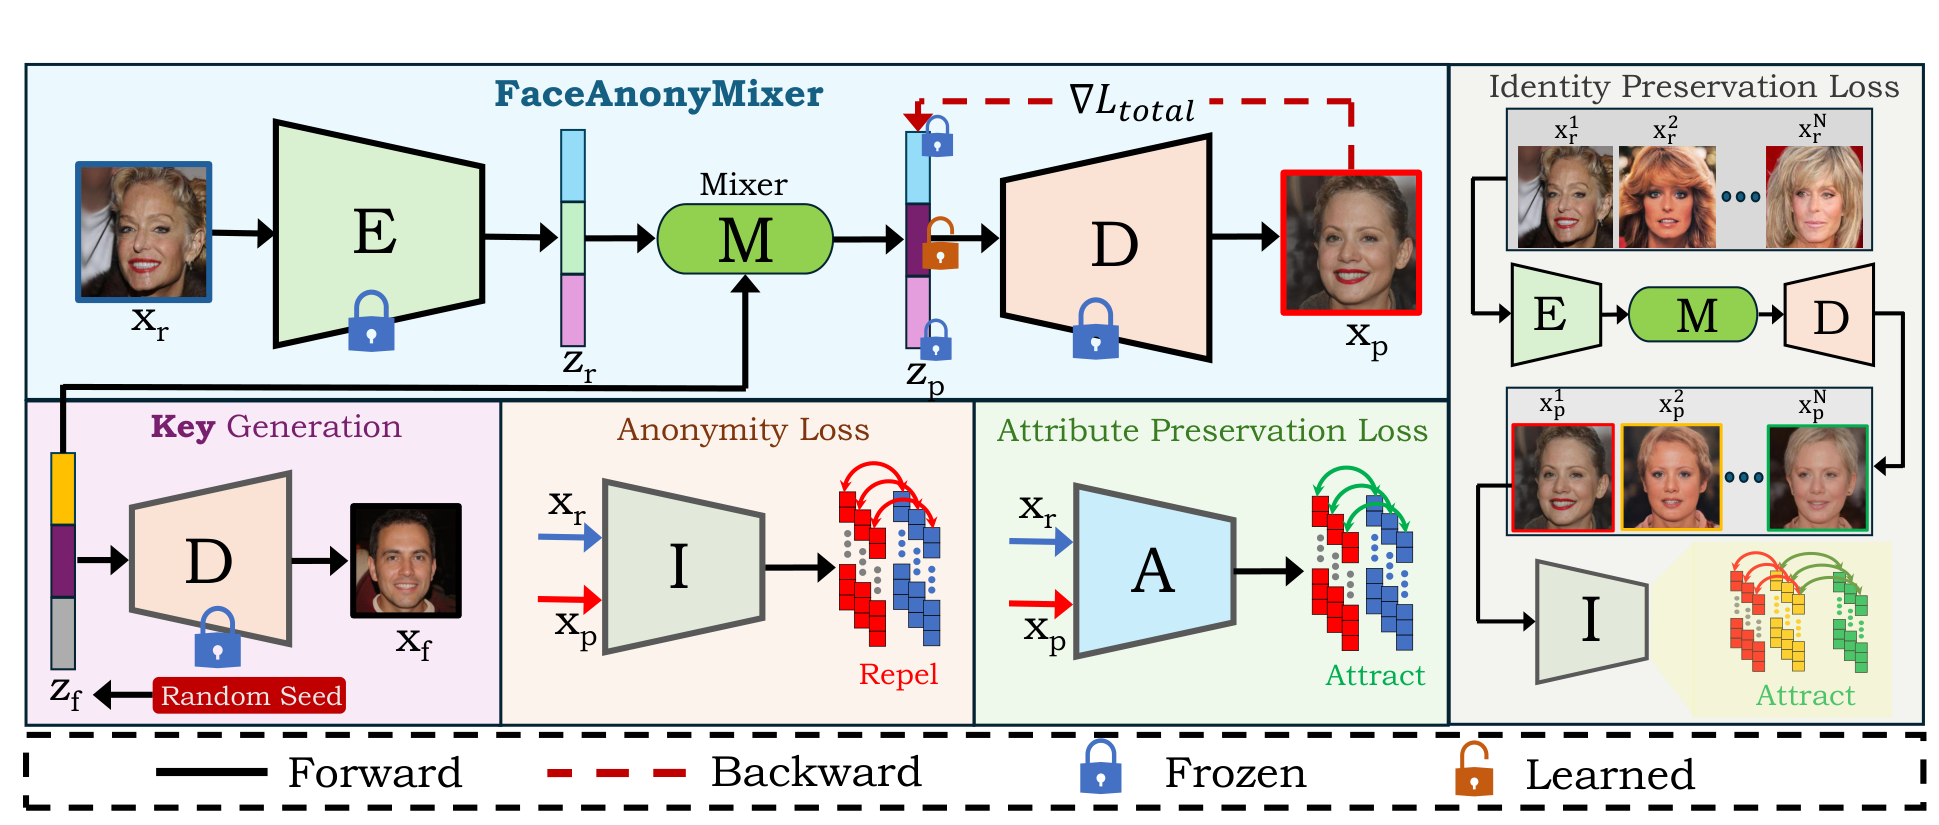
\includegraphics[width=\textwidth]{faceanonymixer-pipeline.png}
\caption[Tổng quan quy trình xử lý của FaceAnonyMixer (Nguồn: Hình 3, bài báo gốc FaceAnonyMixer).]{Tổng quan quy trình xử lý của FaceAnonyMixer. Nguồn: Hình 3, bài báo gốc FaceAnonyMixer \cite{alam2025}.}
\label{fig:faceanonymixer-pipeline}
\end{figure}

\par\medskip\noindent\textbf{Bước 1: Đưa ảnh vào không gian tiềm ẩn}\par\smallskip
Ảnh khuôn mặt thật $\mathbf{x}_r$ được đưa qua bộ mã hóa e4e để thu được mã tiềm ẩn $\mathbf{z}_r \leftarrow \mathbf{E}(\mathbf{x}_r) \in \mathcal{W}^+$ gồm 18 tầng ngữ nghĩa, trong đó các tầng $0\text{--}2$ kiểm soát cấu trúc thô (tư thế, hình dáng mặt), các tầng $3\text{--}7$ biểu diễn đặc trưng định danh và các tầng $8\text{--}17$ lưu giữ chi tiết mịn (kiểu tóc, phông nền).

\par\medskip\noindent\textbf{Bước 2: Ánh xạ khóa}\par\smallskip
Sử dụng khóa có thể hủy $\mathbf{k} \in \mathcal{K}$ làm hạt giống ngẫu nhiên để lấy mẫu một mã tiềm ẩn giả lập từ không gian $\mathcal{W}^+$:
\[
\mathbf{z}_f \leftarrow \mathbf{S}(\mathbf{k}).
\]

\par\medskip\noindent\textbf{Bước 3: Khởi tạo bằng phép trộn thô}\par\smallskip
Thay thế trực tiếp các tầng mang thông tin danh tính ($3\text{--}7$) của $\mathbf{z}_r$ bằng các tầng tương ứng của $\mathbf{z}_f$, đồng thời giữ nguyên các tầng cấu trúc thô và chi tiết nền:
\begin{equation}
\mathbf{z}_p = \mathbf{M}_{\text{naive}}(\mathbf{z}_r, \mathbf{z}_f) = \bigl[\mathbf{z}_r^{(0:2)},\; \mathbf{z}_f^{(3:7)},\; \mathbf{z}_r^{(8:17)}\bigr].
\end{equation}

\par\medskip\noindent\textbf{Bước 4: Tăng cường khả năng nhận dạng}\par\smallskip
Tạo $N$ biến thể tăng cường $\mathbf{x}_r^1, \dots, \mathbf{x}_r^N$ từ $\mathbf{x}_r$ với các tư thế và biểu cảm khác nhau (hoặc sử dụng trực tiếp nhiều ảnh khác nhau của cùng một người nếu có sẵn), sau đó mã hóa $\mathbf{z}_r^i \leftarrow \mathbf{E}(\mathbf{x}_r^i)$ và khởi tạo trộn thô với cùng mã khóa:
\[
\mathbf{z}_p^i \leftarrow \mathbf{M}_{\text{naive}}(\mathbf{z}_r^i, \mathbf{z}_f), \quad i \in \{1, \dots, N\}.
\]

\par\medskip\noindent\textbf{Bước 5: Vòng lặp tối ưu ba hàm mất mát}\par\smallskip
Do sự tách biệt thuộc tính trong $\mathcal{W}^+$ chưa hoàn hảo tuyệt đối, hệ thống tinh chỉnh các mã tiềm ẩn qua $T$ bước lặp ($t = 1, \dots, T$). Tại mỗi bước lặp, trước hết giải mã các ảnh bảo vệ tạm thời từ các mã tiềm ẩn hiện tại: $\mathbf{x}_p \leftarrow \mathbf{D}(\mathbf{z}_p)$ và $\mathbf{x}_p^i \leftarrow \mathbf{D}(\mathbf{z}_p^i)$. Tiếp theo, tính ba thành phần hàm mất mát:
\begin{align}
\mathcal{L}_{\text{anon}} &= \max\Bigl\{0,\; \cos\bigl(\mathbf{I}(\mathbf{x}_p), \mathbf{I}(\mathbf{x}_r)\bigr) - m\Bigr\}, \\
\mathcal{L}_{\text{idp}} &= \frac{1}{N(N-1)} \sum_{i=1}^{N} \sum_{j=i+1}^{N} \bigl\| \mathbf{I}(\mathbf{x}_p^i) - \mathbf{I}(\mathbf{x}_p^j) \bigr\|_2, \\
\mathcal{L}_{\text{attr}} &= \bigl\| \mathbf{A}(\mathbf{x}_p) - \mathbf{A}(\mathbf{x}_r) \bigr\|_1,
\end{align}
trong đó $m$ là siêu tham số lề (đặt $m = 0$ để ép $\mathbf{x}_p$ tiến tới trực giao với $\mathbf{x}_r$ trong không gian danh tính), $\mathcal{L}_{\text{idp}}$ buộc các biến thể cùng người dưới cùng khóa hội tụ gần nhau, còn $\mathcal{L}_{\text{attr}}$ giữ lại các thuộc tính phi danh tính của ảnh gốc. Cuối cùng, tổng mất mát được xác định theo $\mathcal{L}_{\text{total}} = \lambda_1 \mathcal{L}_{\text{anon}} + \lambda_2 \mathcal{L}_{\text{idp}} + \lambda_3 \mathcal{L}_{\text{attr}}$, và các mã tiềm ẩn được cập nhật bằng hạ gradient với tốc độ học $\eta$:
\[
\mathbf{z}_p \leftarrow \mathbf{z}_p - \eta \nabla_{\mathbf{z}_p} \mathcal{L}_{\text{total}}, \qquad \mathbf{z}_p^i \leftarrow \mathbf{z}_p^i - \eta \nabla_{\mathbf{z}_p^i} \mathcal{L}_{\text{total}}.
\]

\par\medskip\noindent\begin{minipage}{\textwidth}
\textbf{Bước 6: Tạo ra ảnh đầu ra}\par\nopagebreak\smallskip
Kết thúc $T$ bước tối ưu, mã tiềm ẩn tối ưu $\mathbf{z}_p$ được đưa qua bộ sinh StyleGAN2 để tạo ra ảnh khuôn mặt bảo vệ hoàn chỉnh $\mathbf{x}_p = \mathbf{D}(\mathbf{z}_p)$.
\end{minipage}
\par
\endgroup

\subsection{Thực nghiệm và kết quả SOTA}
\label{sec::thuc-nghiem}

\subsubsection*{Thiết lập thực nghiệm}
Để kiểm chứng toàn diện cả bốn tiêu chí của chuẩn \textbf{ISO/IEC 24745} \cite{iso24745} (tính khả hủy, tính không thể liên kết, tính không thể đảo ngược và bảo toàn hiệu năng) cùng khả năng ẩn danh và độ chân thực thị giác, bài báo đánh giá FaceAnonyMixer \cite{alam2025} (triển khai trên PyTorch với GPU \textbf{NVIDIA A100 40GB}; tối ưu bằng Adam \cite{kingma2014adam} với $\eta = 0.01$ trong $T = 50$ bước, $N = 5$ biến thể; sử dụng StyleGAN2-FFHQ \cite{karras2020stylegan2}, e4e \cite{tov2021e4e}, ArcFace \cite{deng2019arcface} ResNet50 \cite{he2016resnet} và FaRL \cite{zheng2022farl}) trên hai bộ dữ liệu chuẩn là \textbf{CelebA-HQ} \cite{karras2017celebahq} (tập kiểm thử gồm 1.215 ảnh của 307 danh tính) và \textbf{VGGFace2} \cite{cao2018vggface2} (tập kiểm thử gồm 1.500 ảnh thuộc cùng 307 danh tính để đảm bảo nhất quán). Quá trình đánh giá được thực hiện trên bốn mô hình nhận dạng độc lập (\textbf{IRSE50} \cite{hu2018senet}, \textbf{IR152} \cite{deng2019arcface}, \textbf{FaceNet} \cite{schroff2015facenet}, \textbf{MobileFace} \cite{chen2018mobileface}) tại ba ngưỡng bảo mật tỷ lệ chấp nhận nhầm $\text{FMR} \in \{0.1\%, 0.01\%, 0.001\%\}$, đồng thời sử dụng dịch vụ nhận dạng thương mại \textbf{Face++ API} \cite{facepp2024} để đo điểm tin cậy tương đồng giữa ảnh bảo vệ và ảnh gốc trong điều kiện ứng dụng thực tế, và đối chiếu trực tiếp với phương pháp học sâu tiên tiến trước đó là \textbf{CanFG} \cite{wang2024canfg}.

\subsubsection*{Đánh giá tính ẩn danh và tính không thể liên kết}

\begin{table}[H]
\centering
\scriptsize
\setlength{\tabcolsep}{3.5pt}
\caption[Tỷ lệ bảo vệ thành công PSR đánh giá tính ẩn danh]{Tỷ lệ bảo vệ thành công PSR (\%) đánh giá tính ẩn danh trên CelebA-HQ và VGGFace2 ($\uparrow$ tốt hơn). Nguồn: Bảng 1, bài báo gốc FaceAnonyMixer.}
\label{tab:anonymity_psr}
\resizebox{\textwidth}{!}{%
\begin{tabular}{|l|c|cccc|cccc|c|}
\hline
\multirow{2}{*}{\textbf{Phương pháp}} & \multirow{2}{*}{\textbf{FMR}} & \multicolumn{4}{c|}{\textbf{CelebA-HQ}} & \multicolumn{4}{c|}{\textbf{VGGFace2}} & \multirow{2}{*}{\textbf{Trung bình}} \\
\cline{3-10}
 & & IRSE50 & IR152 & FaceNet & MobileFace & IRSE50 & IR152 & FaceNet & MobileFace & \\
\hline
\multirow{3}{*}{CanFG} & 0.1\% & 71.85 & 70.21 & 81.48 & 34.81 & 1.09 & 15.27 & 30.68 & 0.07 & 38.18 \\
 & 0.01\% & 60.49 & 54.40 & 71.44 & 22.88 & 0.36 & 8.54 & 21.27 & 0.05 & 29.93 \\
 & 0.001\% & 50.37 & 40.00 & 60.58 & 14.65 & 0.14 & 4.20 & 15.85 & 0.01 & 23.22 \\
\hline
\multirow{3}{*}{\textbf{FaceAnonyMixer}} & 0.1\% & \textbf{78.68} & \textbf{95.47} & \textbf{99.51} & \textbf{46.83} & \textbf{98.61} & \textbf{99.07} & \textbf{98.15} & \textbf{93.52} & \textbf{88.73} \\
 & 0.01\% & \textbf{65.58} & \textbf{84.28} & \textbf{97.28} & \textbf{29.14} & \textbf{96.76} & \textbf{97.69} & \textbf{95.37} & \textbf{85.19} & \textbf{81.41} \\
 & 0.001\% & \textbf{61.62} & \textbf{65.68} & \textbf{91.60} & \textbf{24.85} & \textbf{90.67} & \textbf{92.06} & \textbf{88.81} & \textbf{74.09} & \textbf{73.67} \\
\hline
\end{tabular}%
}
\end{table}

\begin{table}[H]
\centering
\scriptsize
\setlength{\tabcolsep}{3.5pt}
\caption[Tỷ lệ bảo vệ thành công PSR đa khóa đánh giá tính không thể liên kết]{Tỷ lệ bảo vệ thành công PSR (\%) đa khóa đánh giá tính không thể liên kết ($\uparrow$ tốt hơn). Nguồn: Bảng 2, bài báo gốc FaceAnonyMixer.}
\label{tab:unlinkability_psr}
\resizebox{\textwidth}{!}{%
\begin{tabular}{|l|c|cccc|cccc|c|}
\hline
\multirow{2}{*}{\textbf{Phương pháp}} & \multirow{2}{*}{\textbf{FMR}} & \multicolumn{4}{c|}{\textbf{CelebA-HQ}} & \multicolumn{4}{c|}{\textbf{VGGFace2}} & \multirow{2}{*}{\textbf{Trung bình}} \\
\cline{3-10}
 & & IRSE50 & IR152 & FaceNet & MobileFace & IRSE50 & IR152 & FaceNet & MobileFace & \\
\hline
\multirow{3}{*}{CanFG} & 0.1\% & 53.50 & 56.13 & 72.51 & 22.80 & 4.36 & 8.83 & 25.18 & 2.41 & 30.72 \\
 & 0.01\% & 40.49 & 39.59 & 58.27 & 11.28 & 2.41 & 4.63 & 16.71 & 1.13 & 21.81 \\
 & 0.001\% & 29.05 & 24.44 & 45.10 & 5.76 & 0.19 & 2.39 & 11.8 & 0.21 & 14.87 \\
\hline
\multirow{3}{*}{\textbf{FaceAnonyMixer}} & 0.1\% & \textbf{86.21} & \textbf{95.56} & \textbf{97.58} & \textbf{47.10} & \textbf{98.35} & \textbf{98.75} & \textbf{97.89} & \textbf{92.20} & \textbf{89.21} \\
 & 0.01\% & \textbf{66.45} & \textbf{77.82} & \textbf{95.56} & \textbf{30.97} & \textbf{95.15} & \textbf{96.14} & \textbf{95.87} & \textbf{85.21} & \textbf{80.40} \\
 & 0.001\% & \textbf{45.08} & \textbf{60.48} & \textbf{91.53} & \textbf{19.27} & \textbf{88.17} & \textbf{90.47} & \textbf{82.69} & \textbf{77.34} & \textbf{69.38} \\
\hline
\end{tabular}%
}
\end{table}

Từ Bảng~\ref{tab:anonymity_psr} và Bảng~\ref{tab:unlinkability_psr}, FaceAnonyMixer vượt trội hoàn toàn CanFG ở mọi mô hình và mọi ngưỡng bảo mật. Cụ thể, khi đặt ngưỡng nhận diện ở mức chỉ cho phép nhận nhầm người lạ $0.1\%$, tỷ lệ hệ thống không nhận ra ảnh bảo vệ là người gốc tăng từ $38.18\%$ lên $88.73\%$ ($+50.55\%$); đồng thời tỷ lệ hai ảnh bảo vệ của cùng một người nhưng khác khóa không bị nhận ra là cùng một người tăng từ $30.72\%$ lên $89.21\%$ ($+58.49\%$). Trên tập dữ liệu phức tạp VGGFace2, CanFG gần như thất bại (tỷ lệ che giấu được danh tính gốc chỉ còn $0.01\%\text{--}30.68\%$), trong khi FaceAnonyMixer vẫn đạt trên $90\%$ ở hầu hết các mô hình. Sự khác biệt này bắt nguồn trực tiếp từ hai thay đổi kiến trúc cốt lõi: (1) CanFG \cite{wang2024canfg} biến đổi trực tiếp trên mạng U-Net \cite{ronneberger2015unet} có liên kết tắt giữ lại nhiều chi tiết không gian của ảnh gốc và thiếu hàm tối ưu trực giao, nên danh tính cũ vẫn bị rò rỉ và các khóa khác nhau cho ra khuôn mặt na ná nhau; (2) ngược lại, FaceAnonyMixer \textbf{thay thế triệt để các tầng danh tính ($3\text{--}7$)} trong không gian $\mathcal{W}^+$ giàu biểu diễn của StyleGAN2 kết hợp hàm $\mathcal{L}_{\text{anon}}$ ép vector đặc trưng tiến tới trực giao với ảnh gốc ($m=0$). Nhờ đó, mỗi khóa $\mathbf{k}$ đưa khuôn mặt sang một danh tính giả độc lập. Bổ sung cho PSR, đánh giá theo khung không thể liên kết Gomez-Barrero \cite{gomezbarrero2017} cho thấy chỉ số liên kết toàn cục $D_{\leftrightarrow}^{\text{sys}}$ giảm sâu từ $0.90$ xuống còn $0.12$ trên CelebA-HQ và từ $0.95$ xuống còn $0.05$ trên VGGFace2, khẳng định khả năng chống đối chiếu chéo mạnh mẽ (minh họa trực quan tại Hình~\ref{fig:qualitative-comparison}).

\begin{figure}[H]
\centering
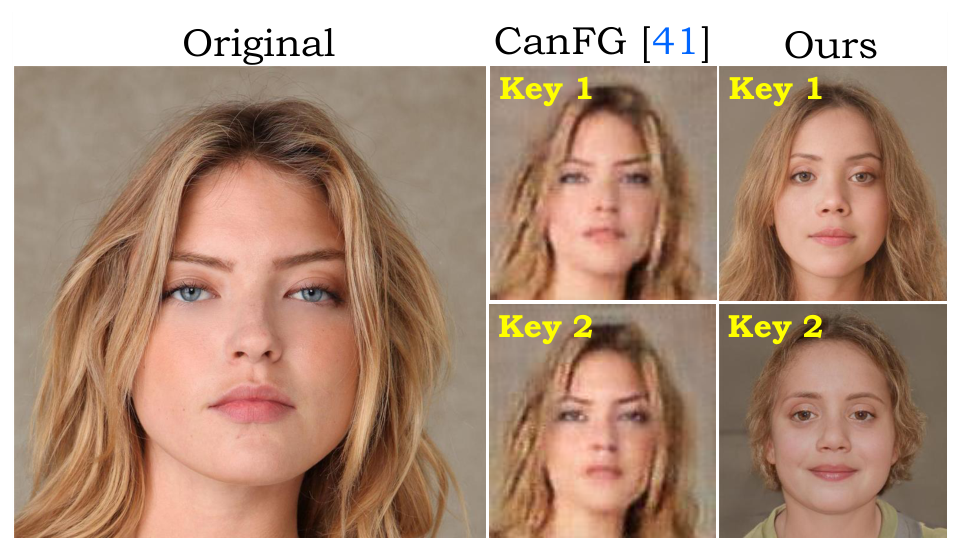
\includegraphics[width=0.76\textwidth]{faceanonymixer-comparison.png}
\caption[So sánh định tính giữa CanFG và FaceAnonyMixer với hai khóa khác nhau (Nguồn: Hình 2, bài báo gốc FaceAnonyMixer).]{So sánh định tính giữa CanFG và FaceAnonyMixer với hai khóa khác nhau: CanFG giữ nhiều nét tương đồng giữa các khóa kèm biến dạng nhiễu, trong khi FaceAnonyMixer tạo khuôn mặt tách biệt và tự nhiên hơn theo từng khóa. Nguồn: Hình 2, bài báo gốc FaceAnonyMixer \cite{alam2025}.}
\label{fig:qualitative-comparison}
\end{figure}

\subsubsection*{Đánh giá thực tế, chống đảo ngược, hiệu năng nhận dạng và độ ổn định khóa}

\begin{table}[H]
\centering
\scriptsize
\setlength{\tabcolsep}{2pt}
\begin{minipage}[t]{0.45\textwidth}
\centering
\caption[Điểm tin cậy tương đồng trên dịch vụ Face++ API]{Điểm tin cậy trên Face++ API ($\downarrow$ tốt hơn). Nguồn: Bảng 3, bài báo gốc.}
\label{tab:facepp}
\resizebox{\linewidth}{!}{%
\begin{tabular}{|l|ccc|}
\hline
\textbf{Phương pháp} & \textbf{CelebA-HQ} & \textbf{VGGFace2} & \textbf{TB} \\
\hline
CanFG & 71.37 & 70.78 & 71.07 \\
\textbf{FaceAnonyMixer} & \textbf{53.73} & \textbf{31.51} & \textbf{58.37} \\
\hline
\end{tabular}%
}
\end{minipage}
\hfill
\begin{minipage}[t]{0.52\textwidth}
\centering
\caption[Hiệu năng xác thực EER và AUC sau bảo vệ]{Hiệu năng xác thực EER ($\downarrow$ tốt hơn) và AUC ($\uparrow$ tốt hơn). Nguồn: Bảng 5, bài báo gốc.}
\label{tab:utility}
\begin{tabular}{|l|cc|cc|}
\hline
\multirow{2}{*}{\textbf{Phương pháp}} & \multicolumn{2}{c|}{\textbf{CelebA-HQ}} & \multicolumn{2}{c|}{\textbf{VGGFace2}} \\
\cline{2-5}
 & EER$\downarrow$ & AUC$\uparrow$ & EER$\downarrow$ & AUC$\uparrow$ \\
\hline
Ảnh gốc & 0.027 & 0.990 & 0.074 & 0.964 \\
CanFG & 0.045 & 0.988 & 0.101 & 0.951 \\
\textbf{FaceAnonyMixer} & \textbf{0.019} & \textbf{0.997} & \textbf{0.059} & \textbf{0.975} \\
\hline
\end{tabular}
\end{minipage}
\end{table}

Các kết quả bổ trợ dưới đây củng cố tính toàn diện của phương pháp:
\begin{itemize}
    \item \textbf{Kiểm tra tính ứng dụng bằng API nhận dạng đời thực (Bảng~\ref{tab:facepp}):} Điểm tin cậy tương đồng trên Face++ giảm từ $71.07$ (CanFG) xuống $58.37$ (riêng VGGFace2 giảm sâu từ $70.78$ còn $31.51$), chứng tỏ việc tối ưu trong $\mathcal{W}^+$ đánh lừa hiệu quả ngay cả các hệ thống thương mại không rõ kiến trúc.
    \item \textbf{Chống đảo ngược ngay cả khi lộ khóa (Bảng~\ref{tab:noninvertibility}, Phụ lục~\ref{app:extra_tables}):} Ngay cả khi kẻ tấn công biết cả khóa $\mathbf{k}$ lẫn ảnh bảo vệ để thay lại tầng giữa hoặc huấn luyện mạng dịch ảnh ngược \textit{pix2pix} \cite{isola2017pix2pix}, tỷ lệ ảnh tái tạo không bị nhận ra là người gốc vẫn đạt $93.80\%\text{--}99.26\%$ tại ngưỡng chỉ cho phép nhận nhầm người lạ $0.1\%$. Lý do là phần mã định danh gốc $\mathbf{z}_r^{(3:7)}$ đã bị loại bỏ hoàn toàn trước khi tối ưu phi tuyến qua 50 bước lặp, khiến ánh xạ ngược trở nên bất khả thi.
    \item \textbf{Bảo toàn nhận dạng và chất lượng ảnh (Bảng~\ref{tab:utility}):} CanFG làm suy giảm khả năng xác thực so với ảnh gốc (EER trên CelebA-HQ tăng từ $0.027 \rightarrow 0.045$; trên VGGFace2 tăng từ $0.074 \rightarrow 0.101$) vì tối ưu đối nghịch trên U-Net không có ràng buộc giữ biểu cảm, hướng nhìn gây méo đặc trưng (FID \cite{heusel2017fid} $= 82.52$). Ngược lại, FaceAnonyMixer giảm EER xuống \textbf{0.019} (CelebA-HQ) và \textbf{0.059} (VGGFace2) --- thậm chí tốt hơn cả ảnh gốc chưa bảo vệ --- nhờ $\mathcal{L}_{\text{idp}}$ gom chặt các ảnh bảo vệ cùng người dưới cùng khóa trong không gian ArcFace, trong khi $\mathcal{L}_{\text{attr}}$ (FaRL) và bộ sinh StyleGAN2 giữ biểu cảm tự nhiên với FID chỉ còn \textbf{37.73}.
    \item \textbf{Ổn định trước sự thay đổi khóa (Bảng~\ref{tab:key_robustness}, Phụ lục~\ref{app:extra_tables}):} Qua $5$ khóa ngẫu nhiên khác nhau, tỷ lệ bảo vệ thành công trên IR152 duy trì trung bình $93.51\%$ với độ lệch chuẩn rất nhỏ (độ lệch chuẩn $= 2.33$), khẳng định hiệu quả bảo vệ không phụ thuộc vào việc chọn khóa đặc biệt.
\end{itemize}

\subsubsection*{Thực nghiệm loại bỏ từng thành phần}
Để đánh giá đóng góp riêng của từng thành phần trong hàm mất mát, tác giả lần lượt loại bỏ từng hàm mục tiêu: khi bỏ hàm bảo toàn danh tính ($\mathcal{L}_{\text{idp}}$), các ảnh của cùng một người dù dùng chung khóa vẫn bị ánh xạ sang các danh tính giả không nhất quán, làm suy giảm rõ rệt độ tin cậy xác thực; khi bỏ hàm bảo toàn thuộc tính ($\mathcal{L}_{\text{attr}}$), ảnh bảo vệ đánh mất các đặc trưng phi danh tính quan trọng như nụ cười và biểu cảm, làm giảm độ chân thực cũng như khả năng dùng cho các tác vụ phụ. Kết hợp với phân tích độ ổn định trên 5 khóa ngẫu nhiên ở trên, nghiên cứu cắt bỏ khẳng định cả ba hàm mất mát đều cần thiết để đồng thời đạt ẩn danh mạnh, nhất quán nhận diện và chất lượng thị giác cao.

% =====================================================================
% TC3. QUAN HỆ GIỮA CHƯƠNG SÁCH VÀ BÀI BÁO
% Nguồn nguyên văn tổng hợp từ các đoạn rải rác:
%   - report/chapter1/1.1-summary.tex (dòng 46--47)
% =====================================================================
\section{Quan hệ giữa chương sách và bài báo}
\label{sec:tc3}

\subsection{Kế thừa và phát triển từ chương sách}
\label{sec:tc3-ke-thua}
FaceAnonyMixer \cite{alam2025} kế thừa trực tiếp tư tưởng của sinh trắc học có thể hủy \cite{adler2008, ratha2001}: biến đổi dữ liệu khuôn mặt theo khóa bí mật riêng cho từng ứng dụng nhằm thu hồi, cấp lại mẫu mới khi bị lộ và ngăn chặn đối chiếu chéo giữa các hệ thống. Đồng thời, bài báo chọn đi theo định hướng sinh đầu ra là ảnh khuôn mặt đã bảo vệ (tương tự phương pháp biến dạng lưới hình học) thay vì chỉ biến đổi trên không gian đặc trưng, sử dụng trực tiếp với các hệ thống nhận dạng chuẩn mà không cần phải điều chỉnh quá nhiều.

% Nguồn nguyên văn: report/chapter1/1.1-summary.tex (dòng 46--47)
Cuốn sách và bài báo chỉ ra hai giới hạn của nhóm biến dạng ảnh trên không gian ảnh: (1) biến dạng lưới mạnh hoặc pha trộn điểm ảnh tạo ra vùng méo phi tự nhiên khiến các bộ nhận dạng hiện đại không trích xuất đặc trưng chính xác được và (2) với phép biến dạng lưới khả nghịch $I_{\mathbf{k}} = I \circ \mathcal{T}_{\mathbf{k}}^{-1}$, nếu lộ khóa $\mathbf{k}$ thì kẻ tấn công có thể dễ dàng giải biến dạng ngược để khôi phục khuôn mặt gốc. Hai hạn chế này là cơ sở để FaceAnonyMixer chuyển sang thao tác trên không gian tiềm ẩn $\mathcal{W}^+$.

Trên nền tảng đó, FaceAnonyMixer phát triển cơ chế bảo vệ mẫu bằng cách tận dụng năng lực tạo sinh của StyleGAN2 và cấu trúc phân tầng tách biệt thuộc tính trong không gian tiềm ẩn $\mathcal{W}^+$. Thay vì biến dạng trực tiếp trên điểm ảnh, phương pháp chỉ thay thế có chọn lọc các tầng chứa thông tin định danh bằng mã sinh từ khóa, đồng thời tận dụng khả năng hòa trộn phong cách của StyleGAN2 để tái tổng hợp khuôn mặt mới tự nhiên, giữ nguyên tư thế, biểu cảm và bối cảnh ảnh mà không cần huấn luyện lại mô hình. Kết hợp cùng tối ưu đa mục tiêu trên không gian tiềm ẩn, bài báo đáp ứng đồng thời bốn yêu cầu của chuẩn ISO/IEC 24745 (tính khả hủy, tính không thể liên kết, tính không thể đảo ngược và bảo toàn hiệu năng), qua đó giải quyết trực tiếp bài toán chống tái tạo ngược và đánh đổi độ chính xác mà Chương~19 từng đặt ra đối với các lược đồ biến dạng cổ điển.

\subsection{Phân tích khác biệt về phương pháp}
\label{sec:tc3-khac-biet}
Dù cùng hướng tới tạo ảnh khuôn mặt có thể hủy để tương thích trực tiếp với các hệ thống nhận dạng sẵn có, kỹ thuật biến dạng lưới hình học trong Chương~19 và FaceAnonyMixer đại diện cho hai cách tiếp cận khác biệt về bản chất xử lý: một bên biến đổi hình học trực tiếp trên lưới tọa độ điểm ảnh, bên còn lại tái tổng hợp khuôn mặt thông qua điều khiển ngữ nghĩa trong không gian tiềm ẩn $\mathcal{W}^+$ của mô hình tạo sinh tiền huấn luyện. Bảng~\ref{tab:book-vs-paper} tóm tắt các khác biệt phương pháp cốt lõi giữa hai cách tiếp cận này.

\begin{table}[H]
\centering
\small
\setlength{\tabcolsep}{4pt}
\renewcommand{\arraystretch}{1.15}
\caption[So sánh khác biệt giữa biến dạng lưới hình học và FaceAnonyMixer]{So sánh khác biệt về phương pháp giữa biến dạng lưới hình học (Chương~19) và bài báo FaceAnonyMixer.}
\label{tab:book-vs-paper}
\begin{tabular}{@{}L{3.2cm}L{5.7cm}L{5.7cm}@{}}
\toprule
\textbf{Khía cạnh} & \textbf{Biến dạng lưới hình học} & \textbf{FaceAnonyMixer} \\
\midrule
\textbf{Không gian xử lý} & Biến dạng trực tiếp trên lưới tọa độ điểm ảnh. & Trộn các tầng danh tính trong không gian tiềm ẩn của StyleGAN2. \\
\textbf{Vai trò của khóa} & Di chuyển lưới cố định theo khóa. & Sinh mã khuôn mặt giả để hòa trộn và tinh chỉnh phi tuyến. \\
\textbf{Chống đảo ngược} & Dễ giải biến dạng ngược nếu lộ khóa. & Xóa thông tin danh tính gốc và tối ưu lặp, không thể khôi phục khi lộ khóa. \\
\textbf{Bảo toàn nhận dạng} & Không có ràng buộc tối ưu; dễ méo ảnh và giảm độ chính xác. & Dùng ba hàm mất mát để vừa ẩn danh, vừa giữ nhận diện và biểu cảm. \\
\textbf{Chi phí triển khai} & Nhẹ, nhanh, không cần mô hình học sâu. & Nặng hơn do tối ưu lặp và phụ thuộc nhiều mô hình tiền huấn luyện. \\
\bottomrule
\end{tabular}
\end{table}

Nhìn chung, bước chuyển từ biến đổi tọa độ sang thao tác có kiểm soát trong không gian tiềm ẩn giúp FaceAnonyMixer giải quyết trực tiếp sự đánh đổi giữa bảo mật và độ tự nhiên của kỹ thuật trong giáo trình, nhưng đồng thời chuyển gánh nặng kỹ thuật sang chi phí suy luận và sự phụ thuộc vào năng lực của các mô hình nền.

% =====================================================================
% TC4. ĐÁNH GIÁ KỸ THUẬT
% Nguồn nguyên văn: report/chapter4/4.2-limitation.tex (dòng 5--21)
% =====================================================================
\section{Đánh giá kỹ thuật}
\label{sec::danh-gia-han-che}

\subsection{Điểm mạnh}
% Nguồn nguyên văn: report/chapter4/4.2-limitation.tex (dòng 5--12)
So với các phép biến đổi hình học trên không gian ảnh như biến dạng lưới hình học, phương pháp \textbf{FaceAnonyMixer} thao tác trong không gian tiềm ẩn của mô hình sinh và đạt được bốn cải tiến chính:
\begin{itemize}\setlength{\itemsep}{2pt}\setlength{\parskip}{0pt}
    \item \textbf{Ảnh tự nhiên và tương thích rộng:} Sinh khuôn mặt chân thực, giữ nguyên biểu cảm và tư thế gốc thay vì bóp méo lưới điểm ảnh, giúp dùng trực tiếp trên các hệ thống nhận dạng chuẩn.
    \item \textbf{Cân bằng bảo mật và độ chính xác:} Giải quyết vấn đề đánh đổi của biến dạng lưới hình học (biến dạng mạnh làm hỏng nhận diện, biến dạng nhẹ dễ lộ danh tính), vừa ẩn danh hiệu quả vừa duy trì khả năng xác thực tương đương ảnh gốc.
    \item \textbf{Chống đảo ngược khi lộ khóa:} Khắc phục điểm yếu dễ bị giải biến dạng của kỹ thuật cổ điển nhờ loại bỏ thông tin định danh gốc và biến đổi phi tuyến trong không gian tiềm ẩn.
    \item \textbf{Đáp ứng ISO/IEC 24745 và linh hoạt đổi khóa:} Tạo danh tính giả tách biệt cho từng khóa để chống đối chiếu chéo, đồng thời không cần huấn luyện lại mô hình khi cấp khóa mới như một số phương pháp học sâu trước đây.
\end{itemize}

\subsection{Hạn chế, giả định và vấn đề còn bỏ ngỏ}
% Nguồn nguyên văn: report/chapter4/4.2-limitation.tex (dòng 15--21)
Bên cạnh các ưu điểm trên, phương pháp và phần thực nghiệm của bài báo vẫn còn một số hạn chế:
\begin{itemize}\setlength{\itemsep}{2pt}\setlength{\parskip}{0pt}
    \item \textbf{Chi phí tính toán cao khi suy luận:} Cơ chế tối ưu lặp cho từng ảnh đầu vào gây độ trễ lớn, khó triển khai thời gian thực hoặc trên thiết bị biên tài nguyên hạn chế.
    \item \textbf{Phụ thuộc vào mô hình nền:} Chất lượng tái tạo phụ thuộc bộ mã hóa đảo ngược và miền ảnh chân dung chuẩn của mô hình sinh, dễ suy giảm khi gặp che khuất nặng hoặc góc nghiêng lớn.
    \item \textbf{Bảo vệ chưa đồng đều giữa các bộ nhận dạng:} Hiệu quả che giấu danh tính vẫn giảm đáng kể trước một số kiến trúc nhận dạng gọn nhẹ nhưng bài báo chưa phân tích rõ nguyên nhân.
    \item \textbf{Thiếu một số đánh giá định lượng:} Chưa công bố số liệu cụ thể về thời gian chạy, bộ nhớ tiêu thụ và hiệu năng trên các tác vụ phụ (nhận diện biểu cảm, ước lượng tuổi).
\end{itemize}

\par\medskip\noindent\textbf{Giả định của phương pháp:} FaceAnonyMixer \cite{alam2025} giả định ảnh khuôn mặt đầu vào đã được phát hiện và căn chỉnh chuẩn (qua MTCNN \cite{zhang2016mtcnn}) phù hợp với miền ảnh chân dung của StyleGAN2 tiền huấn luyện trên FFHQ, đồng thời có đủ nhiều ảnh cùng người hoặc sinh được các biến thể tăng cường hợp lý để áp dụng ràng buộc bảo toàn danh tính. Ngoài ra, quy trình đánh giá mặc định khóa bí mật được quản lý, đồng bộ an toàn giữa khâu đăng ký và xác thực, còn mô hình chống đảo ngược mới xét kẻ tấn công dừng ở mức thay tầng tiềm ẩn hoặc huấn luyện mạng dịch ảnh ngược \textit{pix2pix} \cite{isola2017pix2pix}.

\par\smallskip\noindent\textbf{Vấn đề còn bỏ ngỏ:} Hai vấn đề quan trọng chưa được giải quyết triệt để là sự sụt giảm mạnh tỷ lệ ẩn danh trước các kiến trúc nhận dạng gọn nhẹ (như MobileFace trên tập CelebA-HQ) và khả năng phòng thủ trước các tấn công đảo ngược thích ứng khi kẻ tấn công thu thập được nhiều ảnh bảo vệ của cùng một người. Bên cạnh đó, ảnh hưởng từ thiên lệch dữ liệu của tập FFHQ trong điều kiện chụp tự nhiên phức tạp cũng như khả năng mở rộng khuôn khổ sang hệ thống đa sinh trắc học vẫn là các câu hỏi mở.

% =====================================================================
% TC5. NHẬN XÉT VÀ ĐỀ XUẤT CỦA NHÓM
% Nguồn nguyên văn: report/chapter4/4.2-limitation.tex (dòng 24--35)
% =====================================================================
\section{Nhận xét và đề xuất của nhóm}
\label{sec::de-xuat-cai-tien}

\subsection{Nhận xét về hiệu quả và tính thực tiễn}
Xét về hiệu quả, nhóm đánh giá FaceAnonyMixer \cite{alam2025} nổi bật trước hết ở khả năng tạo ra ảnh khuôn mặt bảo vệ sắc nét, tự nhiên hơn rõ rệt (giữ tốt biểu cảm, tư thế và giảm mạnh FID so với CanFG \cite{wang2024canfg}), tránh được hiện tượng méo hình phi tự nhiên. Quan trọng hơn, phương pháp giải quyết trực tiếp các rào cản kéo dài từ lý thuyết Chương~19 \cite{adler2008} (đánh đổi giữa che giấu danh tính với độ chính xác và nguy cơ tái tạo ngược) cùng điểm yếu dễ giải biến dạng khi lộ khóa của kỹ thuật biến dạng lưới hình học \cite{ratha2001}, đồng thời khắc phục hạn chế của phương pháp hiện đại CanFG như phải huấn luyện lại mỗi khi đổi khóa, che giấu danh tính yếu và dễ bị liên kết chéo --- thể hiện rõ qua EER thấp hơn ảnh gốc và mức giảm sâu điểm tin cậy trên Face++ API \cite{facepp2024}.

Tuy nhiên, về tính thực tiễn, phương pháp chưa phù hợp cho xác thực thời gian thực hay thiết bị do tốn chi phí tối ưu lặp 50 bước trên nhiều mô hình lớn, suy giảm khả năng ẩn danh trước mạng gọn nhẹ như MobileFace và phụ thuộc vào ảnh chân dung căn chỉnh chuẩn. Do đó, FaceAnonyMixer hiện khả thi nhất cho các kịch bản xử lý ngoại tuyến phía máy chủ (như ẩn danh hóa kho ảnh hoặc đăng ký mẫu một lần) trước khi tối ưu tốc độ suy luận cho ứng dụng trực tuyến đại trà.

\subsection{Đề xuất cải tiến và hướng ứng dụng}
% Nguồn nguyên văn: report/chapter4/4.2-limitation.tex (dòng 27--35)
Từ những hạn chế đã phân tích ở mục trên, nhóm đề xuất hai hướng cải tiến kỹ thuật trực tiếp cho FaceAnonyMixer cùng một hướng mở rộng ứng dụng:

\begin{itemize}\setlength{\itemsep}{3pt}\setlength{\parskip}{0pt}
    \item \textbf{Thay vòng lặp tối ưu pha suy luận bằng mạng ánh xạ một lượt:} Điểm yếu lớn nhất của FaceAnonyMixer là phải chạy tối ưu lặp qua nhiều bước cho từng ảnh trên đồng thời StyleGAN2, ArcFace và FaRL. Để khắc phục, có thể huấn luyện trước một mạng ánh xạ nhẹ (chẳng hạn kiến trúc MLP điều kiện theo khóa) nhận đầu vào là cặp mã tiềm ẩn $(\mathbf{z}_r, \mathbf{z}_f)$ để dự đoán trực tiếp phần hiệu chỉnh $\Delta \mathbf{z}_p$ sao cho $\mathbf{z}_p^* = \mathbf{M}_{\text{naive}}(\mathbf{z}_r, \mathbf{z}_f) + \Delta \mathbf{z}_p$ chỉ sau một lần lan truyền xuôi, sử dụng chính tổng mất mát $\mathcal{L}_{\text{total}}$ làm hàm mục tiêu huấn luyện. Vì khóa $\mathbf{z}_f$ đóng vai trò điều kiện đầu vào chứ không gắn cứng vào trọng số mạng, giải pháp này vừa giữ được khả năng đổi khóa không cần huấn luyện lại, vừa giảm đáng kể độ trễ xuống mức gần thời gian thực.

    \item \textbf{Tối ưu ẩn danh trên tập hợp đa bộ trích xuất:} Thực nghiệm cho thấy tỷ lệ ẩn danh trên mạng gọn nhẹ MobileFace ở tập CelebA-HQ giảm mạnh (Bảng~\ref{tab:anonymity_psr}), do mô hình chỉ tối ưu $\mathcal{L}_{\text{anon}}$ dựa trên một bộ trích xuất đơn lẻ là ArcFace (ResNet50) \cite{deng2019arcface} nên chưa xóa hết các đặc trưng cục bộ tần số cao mà các mạng nhẹ thường khai thác. Việc thay thế $\mathbf{I}$ trong $\mathcal{L}_{\text{anon}}$ bằng một tập hợp gồm cả kiến trúc sâu (ResNet \cite{he2016resnet}) và kiến trúc gọn nhẹ (như MobileFaceNet \cite{chen2018mobileface}) sẽ buộc quá trình tối ưu tách biệt danh tính đồng thời trên nhiều không gian đặc trưng khác nhau, nâng cao độ phủ bảo vệ hộp đen.

    \item \textbf{Mở rộng ứng dụng sang ẩn danh hóa dữ liệu và luồng video:} Nhờ giữ được biểu cảm, tư thế gốc thông qua FaRL nhưng vẫn bảo toàn tính phân cụm theo danh tính, FaceAnonyMixer có thể ứng dụng trực tiếp để xây dựng các tập dữ liệu chia sẻ công khai phục vụ bài toán phân tích cảm xúc, hành vi mà không làm lộ danh tính người thật; đồng thời có thể mở rộng cho video bằng cách tối ưu $\mathbf{z}_p^*$ trên các khung hình chính rồi áp dụng đồng nhất cho các khung hình lân cận để đảm bảo tính nhất quán theo thời gian.
\end{itemize}

% =====================================================================
% TÀI LIỆU THAM KHẢO (CHUẨN IEEE)
% Sắp xếp theo đúng thứ tự xuất hiện đầu tiên trong báo cáo (từ TC1 đến Phụ lục B).
% =====================================================================
\clearpage
\phantomsection
\addcontentsline{toc}{section}{Tài liệu tham khảo}
\begin{thebibliography}{99}

\bibitem{adler2008}
A.~Adler, ``Biometric System Security,'' in \textit{Handbook of Biometrics}, A.~K.~Jain, P.~Flynn, and A.~A.~Ross, Eds. Boston, MA, USA: Springer, 2008, ch.~19, pp.~381--402, doi: 10.1007/978-0-387-71041-9\_19.

\bibitem{iso24745}
ISO/IEC JTC1 SC27 Security Techniques, \textit{Information Security, Cybersecurity and Privacy Protection --- Biometric Information Protection}, ISO/IEC Standard 24745:2022, 2022.

\bibitem{ratha2001}
N.~K.~Ratha, J.~H.~Connell, and R.~M.~Bolle, ``Enhancing Security and Privacy in Biometrics-Based Authentication Systems,'' \textit{IBM Syst. J.}, vol.~40, no.~3, pp.~614--634, 2001.

\bibitem{ghafourian2023}
M.~Ghafourian, J.~Fierrez, R.~Vera-Rodriguez, A.~Morales, and I.~Serna, ``OTB-morph: One-Time Biometrics via Morphing,'' \textit{Mach. Intell. Res.}, vol.~20, no.~6, pp.~855--871, 2023.

\bibitem{alam2025}
M.~T.~Alam, F.~Shamshad, F.~Karray, and K.~Nandakumar, ``FaceAnonyMixer: Cancelable Faces via Identity Consistent Latent Space Mixing,'' in \textit{Proc. IEEE Int. Joint Conf. Biometrics (IJCB)}, 2025, pp.~1--10, arXiv:2508.05636. [Online]. Available: \url{https://arxiv.org/abs/2508.05636}

\bibitem{karras2019stylegan}
T.~Karras, S.~Laine, and T.~Aila, ``A Style-Based Generator Architecture for Generative Adversarial Networks,'' in \textit{Proc. IEEE/CVF Conf. Comput. Vis. Pattern Recognit. (CVPR)}, 2019, pp.~4401--4410.

\bibitem{karras2020stylegan2}
T.~Karras, S.~Laine, M.~Aittala, J.~Hellsten, J.~Lehtinen, and T.~Aila, ``Analyzing and Improving the Image Quality of StyleGAN,'' in \textit{Proc. IEEE/CVF Conf. Comput. Vis. Pattern Recognit. (CVPR)}, 2020, pp.~8107--8116.

\bibitem{tov2021e4e}
O.~Tov, Y.~Alaluf, Y.~Nitzan, O.~Patashnik, and D.~Cohen-Or, ``Designing an Encoder for StyleGAN Image Manipulation,'' \textit{ACM Trans. Graph. (TOG)}, vol.~40, no.~4, pp.~1--14, 2021.

\bibitem{kingma2014adam}
D.~P.~Kingma and J.~Ba, ``Adam: A Method for Stochastic Optimization,'' \textit{arXiv preprint arXiv:1412.6980}, 2014.

\bibitem{deng2019arcface}
J.~Deng, J.~Guo, N.~Xue, and S.~Zafeiriou, ``ArcFace: Additive Angular Margin Loss for Deep Face Recognition,'' in \textit{Proc. IEEE/CVF Conf. Comput. Vis. Pattern Recognit. (CVPR)}, 2019, pp.~4690--4699.

\bibitem{he2016resnet}
K.~He, X.~Zhang, S.~Ren, and J.~Sun, ``Deep Residual Learning for Image Recognition,'' in \textit{Proc. IEEE Conf. Comput. Vis. Pattern Recognit. (CVPR)}, 2016, pp.~770--778.

\bibitem{zheng2022farl}
Y.~Zheng \textit{et al.}, ``General Facial Representation Learning in a Visual-Linguistic Manner,'' in \textit{Proc. IEEE/CVF Conf. Comput. Vis. Pattern Recognit. (CVPR)}, 2022, pp.~18697--18709.

\bibitem{karras2017celebahq}
T.~Karras, T.~Aila, S.~Laine, and J.~Lehtinen, ``Progressive Growing of GANs for Improved Quality, Stability, and Variation,'' \textit{arXiv preprint arXiv:1710.10196}, 2017.

\bibitem{cao2018vggface2}
Q.~Cao, L.~Shen, W.~Xie, O.~M.~Parkhi, and A.~Zisserman, ``VGGFace2: A Dataset for Recognising Faces Across Pose and Age,'' in \textit{Proc. 13th IEEE Int. Conf. Automatic Face \& Gesture Recognit. (FG)}, 2018, pp.~67--74.

\bibitem{hu2018senet}
J.~Hu, L.~Shen, and G.~Sun, ``Squeeze-and-Excitation Networks,'' in \textit{Proc. IEEE Conf. Comput. Vis. Pattern Recognit. (CVPR)}, 2018, pp.~7132--7141.

\bibitem{schroff2015facenet}
F.~Schroff, D.~Kalenichenko, and J.~Philbin, ``FaceNet: A Unified Embedding for Face Recognition and Clustering,'' in \textit{Proc. IEEE Conf. Comput. Vis. Pattern Recognit. (CVPR)}, 2015, pp.~815--823.

\bibitem{chen2018mobileface}
S.~Chen, Y.~Liu, X.~Gao, and Z.~Han, ``MobileFaceNets: Efficient CNNs for Accurate Real-Time Face Verification on Mobile Devices,'' in \textit{Proc. Chin. Conf. Biometric Recognit. (CCBR)}, Springer, 2018, pp.~428--438.

\bibitem{facepp2024}
MEGVII Technology, ``Face++ Cognitive Services,'' 2024. [Online]. Available: \url{https://www.faceplusplus.com/}

\bibitem{wang2024canfg}
T.~Wang, Y.~Zhang, X.~Xiao, L.~Yuan, Z.~Xia, and J.~Weng, ``Make Privacy Renewable! Generating Privacy-Preserving Faces Supporting Cancelable Biometric Recognition,'' in \textit{Proc. 32nd ACM Int. Conf. Multimedia}, 2024, pp.~10268--10276, doi: 10.1145/3664647.3680704.

\bibitem{ronneberger2015unet}
O.~Ronneberger, P.~Fischer, and T.~Brox, ``U-Net: Convolutional Networks for Biomedical Image Segmentation,'' in \textit{Proc. Int. Conf. Med. Image Comput. Comput.-Assist. Interv. (MICCAI)}, Springer, 2015, pp.~234--241.

\bibitem{gomezbarrero2017}
M.~Gomez-Barrero, J.~Galbally, C.~Rathgeb, and C.~Busch, ``General Framework to Evaluate Unlinkability in Biometric Template Protection Systems,'' \textit{IEEE Trans. Inf. Forensics Security}, vol.~13, no.~6, pp.~1406--1420, Jun. 2017.

\bibitem{isola2017pix2pix}
P.~Isola, J.-Y.~Zhu, T.~Zhou, and A.~A.~Efros, ``Image-to-Image Translation with Conditional Adversarial Networks,'' in \textit{Proc. IEEE Conf. Comput. Vis. Pattern Recognit. (CVPR)}, 2017, pp.~5967--5976.

\bibitem{heusel2017fid}
M.~Heusel, H.~Ramsauer, T.~Unterthiner, B.~Nessler, and S.~Hochreiter, ``GANs Trained by a Two Time-Scale Update Rule Converge to a Local Nash Equilibrium,'' in \textit{Advances in Neural Information Processing Systems (NeurIPS)}, vol.~30, 2017.

\bibitem{zhang2016mtcnn}
K.~Zhang, Z.~Zhang, Z.~Li, and Y.~Qiao, ``Joint Face Detection and Alignment Using Multitask Cascaded Convolutional Networks,'' \textit{IEEE Signal Process. Lett.}, vol.~23, no.~10, pp.~1499--1503, Oct. 2016.

\bibitem{teoh2006}
A.~B.~J.~Teoh, A.~Goh, and D.~C.~L.~Ngo, ``Random Multispace Quantization as an Analytic Mechanism for BioHashing of Biometric and Random Identity Inputs,'' \textit{IEEE Trans. Pattern Anal. Mach. Intell.}, vol.~28, no.~12, pp.~1892--1901, Dec. 2006, doi: 10.1109/TPAMI.2006.250.

\bibitem{rathgeb2013}
C.~Rathgeb, F.~Breitinger, and C.~Busch, ``Alignment-Free Cancelable Iris Biometric Templates Based on Adaptive Bloom Filters,'' in \textit{Proc. Int. Conf. Biometrics (ICB)}, 2013, pp.~1--8, doi: 10.1109/ICB.2013.6612976.

\bibitem{shahreza2023mlp}
H.~O.~Shahreza, V.~Krivoku{\'c}a Hahn, and S.~Marcel, ``MLP-Hash: Protecting Face Templates via Hashing of Randomized Multi-Layer Perceptron,'' in \textit{Proc. 31st Eur. Signal Process. Conf. (EUSIPCO)}, 2023, pp.~605--609, doi: 10.23919/EUSIPCO58844.2023.10289780.

\bibitem{hukkelas2019}
H.~Hukkel{\r{a}}s, R.~Mester, and F.~Lindseth, ``DeepPrivacy: A Generative Adversarial Network for Face Anonymization,'' in \textit{Proc. Int. Symp. Visual Comput. (ISVC)}, Springer, 2019, pp.~565--578.

\bibitem{maximov2020}
M.~Maximov, I.~Elezi, and L.~Leal-Taix{\'e}, ``CIAGAN: Conditional Identity Anonymization Generative Adversarial Networks,'' in \textit{Proc. IEEE/CVF Conf. Comput. Vis. Pattern Recognit. (CVPR)}, 2020, pp.~5446--5455, doi: 10.1109/CVPR42600.2020.00549.

\bibitem{torkz2019}
R.~Torkzadehmahani, P.~Kairouz, and B.~Paten, ``DP-CGAN: Differentially Private Synthetic Data and Label Generation,'' in \textit{Proc. IEEE/CVF Conf. Comput. Vis. Pattern Recognit. Workshops (CVPRW)}, 2019, pp.~98--104, doi: 10.1109/CVPRW.2019.00018.

\end{thebibliography}

% =====================================================================
% PHỤ LỤC
% =====================================================================
\clearpage
\appendix

% Phụ lục A (Nguồn nguyên văn: report/Appendix/appendix1.tex)
\section{Số liệu thực nghiệm bổ sung}
\label{app:extra_tables}

Phụ lục này trình bày chi tiết hai bảng số liệu thực nghiệm bổ trợ của phương pháp FaceAnonyMixer được trích từ bài báo gốc, bao gồm khả năng chống tấn công đảo ngược khi lộ khóa (Bảng~\ref{tab:noninvertibility}) và độ ổn định qua các khóa ngẫu nhiên (Bảng~\ref{tab:key_robustness}).

\begin{table}[H]
\centering
\small
\setlength{\tabcolsep}{6pt}
\caption[Tỷ lệ bảo vệ thành công PSR chống tấn công đảo ngược khi lộ khóa]{Tỷ lệ bảo vệ thành công PSR (\%) chống tấn công đảo ngược ngay cả khi lộ khóa ($\uparrow$ tốt hơn). Nguồn: Bảng 4, bài báo gốc FaceAnonyMixer.}
\label{tab:noninvertibility}
\begin{tabular}{|l|c|cccc|}
\hline
\textbf{Bộ dữ liệu} & \textbf{FMR} & IRSE50 & IR152 & FaceNet & MobileFace \\
\hline
\multirow{3}{*}{CelebA-HQ} & 0.1\% & 98.02 & 98.77 & 99.26 & 96.79 \\
 & 0.01\% & 94.57 & 97.53 & 96.79 & 88.97 \\
 & 0.001\% & 87.74 & 92.02 & 93.50 & 74.24 \\
\hline
\multirow{3}{*}{VGGFace2} & 0.1\% & 97.60 & 98.40 & 99.15 & 93.80 \\
 & 0.01\% & 94.18 & 97.01 & 95.12 & 86.57 \\
 & 0.001\% & 91.35 & 95.27 & 93.8 & 75.98 \\
\hline
\end{tabular}
\end{table}

\begin{table}[H]
\centering
\small
\setlength{\tabcolsep}{6pt}
\caption[Tỷ lệ bảo vệ thành công PSR theo 5 khóa ngẫu nhiên trên IR152]{Tỷ lệ bảo vệ thành công PSR (\%) theo 5 khóa ngẫu nhiên trên IR152 ($\uparrow$ tốt hơn). Nguồn: Bảng 6, bài báo gốc FaceAnonyMixer.}
\label{tab:key_robustness}
\begin{tabular}{|c|ccccc|c|}
\hline
 & $k_1$ & $k_2$ & $k_3$ & $k_4$ & $k_5$ & \textbf{Độ lệch chuẩn} \\
\hline
PSR & 95.47 & 90.47 & 91.91 & 96.84 & 92.87 & 2.33 \\
\hline
\end{tabular}
\end{table}

% Phụ lục B (Nguồn nội dung: report/chapter3/3.2.5-comparison-table.tex; trình bày tách 2 bảng mô tả ngắn gọn, không ký hiệu)
\clearpage
\section{Bảng so sánh tổng hợp các phương pháp CFB}
\label{sec:cfb-comparison}

Để dễ quan sát trên khổ giấy dọc, bảng tổng hợp các phương pháp sinh trắc khuôn mặt có thể hủy được trình bày thành hai bảng nối tiếp: Bảng~\ref{tab:cfb-comparison} đối chiếu không gian thao tác, khả năng tương thích và chất lượng thị giác; Bảng~\ref{tab:cfb-comparison-iso} đối chiếu mức độ đáp ứng bốn tiêu chí bảo mật của chuẩn ISO/IEC 24745.

\begin{table}[H]
\centering
\caption[So sánh các phương pháp CFB (Phần 1: Không gian, tương thích và chất lượng)]{So sánh các phương pháp sinh trắc khuôn mặt có thể hủy (Phần 1: Không gian thao tác, tính tương thích và chất lượng thị giác).}
\label{tab:cfb-comparison}
\begin{spacing}{1.08}
\footnotesize
\setlength{\tabcolsep}{4pt}
\begin{tabular}{@{}P{3.1cm}P{2.6cm}P{3.0cm}P{3.0cm}P{2.9cm}@{}}
\toprule
\textbf{Phương pháp} & \textbf{Không gian thao tác} & \textbf{Tương thích hệ thống FR} & \textbf{Chất lượng thị giác} & \textbf{Mức độ bảo vệ danh tính} \\
\midrule
BioHashing \cite{teoh2006} & Đặc trưng sang mã nhị phân. & Cần bộ so khớp Hamming riêng. & Không sinh ảnh, chỉ lưu mã. & Chưa đánh giá. \\
\addlinespace[4pt]
Adaptive Bloom filter \cite{rathgeb2013} & Mã nhị phân sang bộ lọc Bloom. & Cần bộ so khớp riêng trên bộ lọc Bloom. & Không sinh ảnh, chỉ lưu mã. & Chưa đánh giá. \\
\addlinespace[4pt]
Block permutation \cite{ratha2001} & Ảnh trực tiếp trên miền điểm ảnh. & Dùng trực tiếp trên hệ thống FR có sẵn. & Ảnh vỡ khối, thiếu tự nhiên, dễ bị phát hiện. & Chưa đánh giá. \\
\addlinespace[4pt]
Image morphing \cite{ghafourian2023} & Ảnh trực tiếp trên miền điểm ảnh. & Dùng trực tiếp trên hệ thống FR có sẵn. & Có vùng méo ảnh, hạn chế tính khả dụng. & Chưa đánh giá. \\
\addlinespace[4pt]
MLP-Hash \cite{shahreza2023mlp} & Đặc trưng qua mạng MLP ngẫu nhiên. & Cần bộ so khớp Hamming riêng. & Không sinh ảnh, chỉ lưu mã. & Chưa đánh giá. \\
\addlinespace[4pt]
DeepPrivacy \cite{hukkelas2019} / CIAGAN \cite{maximov2020} & Ảnh qua mạng GAN có điều kiện. & Chỉ dùng cho phát hiện, không hỗ trợ xác thực. & Giữ tốt tư thế và nền ở độ phân giải thấp. & Thay thế trực tiếp đặc trưng danh tính. \\
\addlinespace[4pt]
DP-CGAN \cite{torkz2019} & Ảnh qua mạng GAN riêng tư vi phân. & Không áp dụng vì chỉ thử trên MNIST. & Riêng tư vi phân làm giảm chất lượng ảnh. & Chưa đánh giá. \\
\addlinespace[4pt]
CanFG \cite{wang2024canfg} & Đặc trưng ArcFace sang ảnh qua U-Net. & Xác thực cần bộ trích xuất VID riêng. & Chất lượng chưa ổn định, FID cao khi kiểm thử chéo. & Hiệu quả che giấu giảm mạnh khi kiểm thử chéo. \\
\midrule
\textbf{FaceAnonyMixer} \cite{alam2025} & Không gian tiềm ẩn của StyleGAN2. & Dùng trực tiếp với hệ thống FR và API thương mại. & Ảnh chân thực, sắc nét, FID thấp. & Tỷ lệ bảo vệ danh tính cao, vượt trội CanFG. \\
\bottomrule
\end{tabular}
\end{spacing}
\end{table}

\begin{table}[H]
\centering
\caption[So sánh các phương pháp CFB (Phần 2: Đáp ứng chuẩn ISO/IEC 24745)]{So sánh các phương pháp sinh trắc khuôn mặt có thể hủy (Phần 2: Đáp ứng bốn tiêu chí bảo mật theo chuẩn ISO/IEC 24745).}
\label{tab:cfb-comparison-iso}
\begin{spacing}{1.08}
\footnotesize
\setlength{\tabcolsep}{4pt}
\begin{tabular}{@{}P{3.1cm}P{2.7cm}P{3.0cm}P{2.8cm}P{3.0cm}@{}}
\toprule
\textbf{Phương pháp} & \textbf{Hủy \& cấp khóa mới} & \textbf{Tính không thể liên kết} & \textbf{Tính không thể đảo ngược} & \textbf{Bảo toàn hiệu năng nhận dạng} \\
\midrule
BioHashing \cite{teoh2006} & Đổi token ngẫu nhiên để tạo mẫu mới. & Tốt khi khóa độc lập nhưng còn tranh cãi giữa các nguồn. & Dễ bị tấn công khôi phục khi lộ khóa. & Tốt khi giữ bí mật khóa, giảm khi dùng chung khóa. \\
\addlinespace[4pt]
Adaptive Bloom filter \cite{rathgeb2013} & Thu hồi bằng cách đổi khóa bí mật. & Dễ bị tấn công liên kết chéo với tỷ lệ cao. & Chỉ đảm bảo một chiều khi dữ liệu phân bố đều. & Chưa đánh giá. \\
\addlinespace[4pt]
Block permutation \cite{ratha2001} & Đổi khóa hoán vị để cấp mẫu mới. & Chưa đánh giá. & Phép hoán vị có thể giải ngược khi lộ khóa. & Làm giảm độ chính xác nhận dạng. \\
\addlinespace[4pt]
Image morphing \cite{ghafourian2023} & Thay đổi khóa theo từng lần sử dụng. & Chưa đánh giá. & Chưa đánh giá. & Lỗi méo ảnh làm hạn chế hiệu năng thực tế. \\
\addlinespace[4pt]
MLP-Hash \cite{shahreza2023mlp} & Đổi mạng MLP ngẫu nhiên theo người dùng. & Đạt mức không thể liên kết tốt. & Vẫn chịu rủi ro khôi phục đáng kể khi lộ khóa. & Tốt khi giữ bí mật khóa, giảm khi dùng chung khóa. \\
\addlinespace[4pt]
DeepPrivacy \cite{hukkelas2019} / CIAGAN \cite{maximov2020} & Không hỗ trợ khóa để thu hồi. & Không xét được do không dùng khóa. & Bộ sinh không tiếp xúc trực tiếp điểm ảnh mặt gốc. & Không hỗ trợ xác thực vì danh tính không gắn khóa. \\
\addlinespace[4pt]
DP-CGAN \cite{torkz2019} & Không hỗ trợ khóa để thu hồi. & Không xét được do không dùng khóa. & Chưa đánh giá. & Không áp dụng vì chỉ đo phân loại MNIST. \\
\addlinespace[4pt]
CanFG \cite{wang2024canfg} & Hủy được nhưng phải huấn luyện lại mô hình. & Ảnh sinh từ các khóa khác nhau vẫn khá giống nhau. & Có nguy cơ bị phá nếu lộ mô hình và bộ VID. & Bảo toàn tốt nhờ phép biến đổi trực giao. \\
\midrule
\textbf{FaceAnonyMixer} \cite{alam2025} & Không cần huấn luyện lại, chỉ tối ưu lại mã tiềm ẩn. & Khả năng chống liên kết chéo cao giữa các khóa. & Không thể tái tạo ảnh gốc ngay cả khi lộ khóa. & Duy trì hiệu năng xác thực rất tốt, EER thấp hơn ảnh gốc. \\
\bottomrule
\end{tabular}
\end{spacing}
\end{table}

% Phụ lục C (Bắt buộc theo Mục 3.8 yêu cầu Seminar 1; nguồn: phancong.md)
\clearpage
\section{Bảng phân công và tỷ lệ đóng góp của từng thành viên}
\label{app:contribution}

\begin{table}[H]
\centering
\caption[Bảng phân công công việc và tỷ lệ đóng góp của Nhóm 9]{Bảng phân công công việc, tiến độ hoàn thành và tỷ lệ đóng góp của các thành viên Nhóm 9.}
\label{tab:contribution}
\begin{spacing}{1.1}
\small
\setlength{\tabcolsep}{4pt}
\begin{tabular}{@{}cP{2.9cm}P{6.8cm}c>{\centering\arraybackslash}p{1.6cm}@{}}
\toprule
\textbf{MSSV} & \textbf{Họ và tên} & \textbf{Phân công} & \textbf{Tiến độ} & \textbf{Tỷ lệ đóng góp} \\
\midrule
23120146 & Hoàng Ngọc & Phụ trách phần phát biểu bài toán, mô tả từng bước phương pháp bài báo, danh mục thuật ngữ/ký hiệu và tổng hợp báo cáo LaTeX. & 100\% & 20\% \\
\addlinespace[4pt]
23120097 & Võ Tất Toàn & Trình bày tổng quan bối cảnh Chương 19 (tối đa 1 trang); nêu vị trí bài toán và liên kết 4 tiêu chuẩn ISO/IEC 24745; trình bày ý tưởng, mô hình toán học và các bước thuật toán Grid Morphing (Ratha et al., 2001). & 100\% & 20\% \\
\addlinespace[4pt]
23120165 & Lê Đức Thành & Nhận xét thực nghiệm \& kết quả SOTA, đánh giá hạn chế, ưu điểm và đề xuất cải tiến. & 100\% & 20\% \\
\addlinespace[4pt]
23120270 & Lê Quốc Hưng & Viết phần Related Work cho chủ đề CFB kèm trích dẫn gốc (nhóm feature-based, image-based, ML/DL tạo sinh và CanFG); lập bảng tổng hợp so sánh các phương pháp tiêu biểu theo 8 tiêu chí. & 100\% & 20\% \\
\addlinespace[4pt]
23120096 & Nguyễn Viết Toàn & Phân tích ưu nhược điểm của Grid Morphing (4 chuẩn ISO, tương thích FR, đánh đổi độ chính xác--bảo mật); tổng hợp các cải tiến và khoảng trống nghiên cứu (gap); phân tích mối quan hệ \& cơ chế cải thiện của FaceAnonyMixer so với Grid Morphing và CanFG. & 100\% & 20\% \\
\midrule
\multicolumn{4}{r}{\textbf{Tổng tỷ lệ đóng góp}} & \textbf{100\%} \\
\bottomrule
\end{tabular}
\end{spacing}
\end{table}

% Phụ lục D (Bắt buộc theo Mục 3.8 & Mục 5 yêu cầu Seminar 1)
\clearpage
\section{Khai báo sử dụng công cụ AI}
\label{app:ai_declaration}

\noindent\textbf{Công cụ AI đã sử dụng:} Google Gemini Argon (Antigravity) và OpenAI Codex.

Nhóm sử dụng công cụ AI với vai trò hỗ trợ tìm hiểu tài liệu, trình bày LaTeX và rà soát tính đầy đủ của báo cáo. Chi tiết mục đích, phạm vi sử dụng và cách nhóm kiểm chứng được tổng hợp trong Bảng~\ref{tab:ai_declaration}.

\begin{table}[H]
\centering
\caption[Tổng hợp mục đích và phạm vi sử dụng công cụ AI]{Tổng hợp mục đích và phạm vi sử dụng công cụ AI của Nhóm 9.}
\label{tab:ai_declaration}
\begin{spacing}{1.02}
\footnotesize
\setlength{\tabcolsep}{4pt}
\begin{tabular}{@{}P{3.3cm}P{6.8cm}P{4.9cm}@{}}
\toprule
\textbf{Nhóm công việc} & \textbf{Mục đích hỗ trợ của AI} & \textbf{Phạm vi \& kiểm chứng của nhóm} \\
\midrule
Tìm hiểu tổng quan tài liệu và thuật ngữ & Tổng hợp, tóm tắt sơ bộ nội dung Chương~19 để nắm tổng quan trước khi đọc chi tiết; giải thích ngắn gọn mục tiêu bài báo; giải thích các khái niệm nền (không gian tiềm ẩn, bốn tiêu chuẩn ISO/IEC 24745) và cơ chế hoạt động của StyleGAN nhằm hiểu lý do tác giả tận dụng. & Áp dụng cho Mục~1 và Mục~2; nhóm đối chiếu trực tiếp với giáo trình và bài báo gốc. \\
\addlinespace[2.5pt]
Hiểu quy trình và công thức toán học & Giải thích, cho ví dụ minh họa quy trình xử lý của tác giả và phân tích ý nghĩa công thức của ba hàm mất mát. & Áp dụng cho Mục~2; nhóm tự kiểm tra lại từng công thức và ký hiệu theo bài báo gốc. \\
\addlinespace[2.5pt]
Tham khảo đánh giá hạn chế và đề xuất & Tổng hợp các hạn chế của mô hình và gợi ý tham khảo các hướng đề xuất cải tiến. & Áp dụng cho Mục~4 và Mục~5; nhóm tự chọn lọc lập luận, đối chiếu số liệu thực nghiệm và tự viết nhận xét. \\
\addlinespace[2.5pt]
Chỉnh sửa câu chữ, trình bày LaTeX và danh mục & Hỗ trợ viết ký hiệu, biểu thức toán học gọn đẹp, căn lề và trình bày bảng LaTeX; hỗ trợ tổng hợp danh sách ký hiệu, thuật ngữ và nháp một số đoạn trình bày phương pháp. & Với bảng thuật ngữ/ký hiệu, nhóm tự điền phần giải thích và giải nghĩa tiếng Việt. Do đoạn văn AI gợi ý thường dài và khó theo dõi trọng tâm, nhóm chủ yếu tự viết lại theo ý hiểu, chỉ giữ lại một số đoạn phù hợp và chỉnh sửa lại câu chữ. \\
\addlinespace[2.5pt]
Rà soát cấu trúc và độ đầy đủ & Kiểm tra đối chiếu báo cáo với các yêu cầu của Seminar~1 để phát hiện các mục còn thiếu. & Áp dụng trên toàn báo cáo; nhóm tự hoàn thiện và chịu trách nhiệm toàn bộ nội dung nộp. \\
\bottomrule
\end{tabular}
\end{spacing}
\end{table}

\par\vspace{2pt}\noindent\textbf{Cam kết của nhóm:} Ngoài các nội dung hỗ trợ đã liệt kê trong Bảng~\ref{tab:ai_declaration}, toàn bộ các phần còn lại của báo cáo đều do các thành viên tự viết và tham khảo trực tiếp từ giáo trình cùng bài báo gốc. Mọi nội dung có tham khảo công cụ AI đều đã được nhóm đọc hiểu, kiểm chứng lại và được kiểm tra trước khi nộp.

\end{document}
